\chapter{Hardware Implementation}
\label{chap:Field}

Previous chapters (chapter \ref{chap:IS}, chapter \ref{chap:US} and chapter \ref{chap:HS}) focussed on characterizing the performance of different CR systems jointly in terms of interference power received by the primary receiver and throughput at the secondary receiver by taking the estimation of the involved channels into account. In addition, it is motivated that the low complexity and the versatility towards unknown primary user signals requirements can be satisfied by employing unconventional channel estimation techniques such as received power-based estimation for acquiring the knowledge of the interacting channels, particularly the channels between the primary and the secondary systems. However, the aforementioned analysis in the previous chapters has been limited to the theoretical expressions. This chapter complements the performance analysis by deploying the proposed channel estimation techniques on a hardware. In this sense, the feasibility of the assumptions considered while deriving the analytical expressions can be examined, thereby facilitating the evolution of the proposed framework. With no loss of generality, an underlay system is considered for the deployment.    
%\begin{abstract}        % give a summary of your paper
%Cognitive radio is one of the potential contenders that address the problem of spectrum scarcity by making efficient use of the currently allocated spectrum below \SI{6}{GHz}. A secondary access to the licensed spectrum is only possible, if the cognitive radio systems restrict the interference to the primary systems. However, the performance analysis of such a cognitive radio system is a challenging task. Currently, performance evaluation of underlay systems is limited to theoretical analysis. Most of the existing theoretical investigations make certain assumptions in order to sustain analytical tractability, which could be unrealistic from the deployment perspective. Motivated by this fact, in this work, we validate the performance of an underlay system by means of laboratory measurements, and consequently propose a hardware demonstrator of such a system. Moreover, we present a graphical user interface to provide insights to the working of the proposed demonstrator and highlight the main issues faced during this experimental study.
%\blfootnote{This work was partially supported by the National Research Fund, Luxembourg under the CORE projects "SeMIGod" and "SATSENT".} 

% please supply keywords within your abstract
%\keywords {Cognitive Relay, underlay system, power control, dynamic access, empirical validation, demonstrator}
%\end{abstract}



%\section{Related Work}

%The amount of data transmitted over wireless channels is constantly increasing. However, the available spectrum is scarce and expensive, with more and more operators competing for their share of it. Therefore, ways have to be found to use the available spectrum more efficiently. Cognitive radio networks do so by enabling dynamic spectrum access to multiple systems. Secondary access to the licensed spectrum has been extensively investigated in the literature and is mainly categorized in terms of three cognitive radio paradigms \cite{Goldsmith09}: 
%\begin{enumerate}
%	\item An interweave system exploits time gaps in the spectrum of primary users for data transmission. 
%	\item An overlay system involves higher network layers to employ advanced coding algorithms to transmit data simultaneously with other systems. 
%	\item In an underlay system, spectrum access is enabled only if the interference power received at primary users is below a certain amount. This can be achieved, for instance, by employing a power control mechanism at the secondary transmitter. 
%\end{enumerate}

%The existing investigations in \cite{Ghasemi07, Xin09, Musa09} depicted the performance limits in terms of throughput achieved at the secondary receiver for the underlay system. However, the performance evaluation has been limited to theoretical analysis, which tends to make certain assumptions (for instance, perfect knowledge of channel), that are not applicable in hardware implementations \cite{Sharma15}. Recently, hardware implementations in context to cognitive radio systems have started to receive significant attention \cite{Ngu13, Anas12, Combes15}, however these deployments are mainly concerned with the interweave system. In this regard, we provide insights for the deployment of underlay systems, in this paper. More specifically, we extend the mathematical framework derived in \cite{Kaushik15} to validate the performance of underlay systems by means of experimental analysis. To complement the analysis presented in \cite{Kaushik15}, 

This chapter provides the following contributions:
\begin{itemize}
	\item Empirical validation: The performance of the underlay systems subject to the employment of received power-based between the PR and the ST is validated by means of a hardware deployment. The variations (induced due to incorporation of channel estimation) in the system parameters are validated by comparing their probability density functions obtained from the measurements to the one computed analytically. Moreover, the joint performance of the underlay system is validated in terms of estimation-throughput tradeoff proposed in chapter \ref{chap:US}. %A suitable hardware environment is establish to perform measurements and evaluate their results by comparing them with the theoretical expressions.
	\item Demonstrator: Upon validating the theoretical expressions, a hardware demonstrator following the guidelines of an underlay system is deployed. In this context, the applicability of the proposed framwork in realistic scenarios can be justified. A graphical user interference is designed to procure insights to the working of the demonstrator.	
\end{itemize}

%This paper is organized as follows: Section \ref{sysmod} introduces the system model. Section \ref{val} describes the experimental setup and the validation of the mathematical model. Section \ref{demo} portrays the implementation of the underlay system's hardware demonstrator. Finally, Section \ref{con} concludes the paper.


\section{System Model}
\label{sysmod}

\subsection{Simplifications}
\label{ssec:simp1}
In contrast to the framework presented in chapter \ref{chap:US}, the following simplifications and modifications are considered for the hardware implementation.
\begin{itemize}
\item The channel estimation (received power-based) is only deployed for the link between the PR and the ST, which is associated with the regulation of the interference (power) received at the PR. In order to simplify the deployment, the interference from the PTs at the SR is neglected. In addition, perfect knowledge of the access channel between the ST and the SR that employs the pilot-based channel estimation is considered\footnote{Since the effect due to the pilot-based channel estimation in terms of time allocated within the frame structure and the amount of variations induced has negligible effect on the performance degradation of the CR system, perfect channel estimation for access channel is a valid argument.}.  
\item The measurements for the validation and the demonstrator consider the deterministic behaviour of the interference channel.  
\item In contrast to the outage constraint proposed in chapter \ref{chap:US}, a confidence probability constraint is employed for capturing the variations due to channel estimation around the interference temperature. %Moreover, previous analysis considers the realization of the power control over multiple frame. Here, the power control subject  
\item Lastly, in contrast to the OFDM signal considered in chapter \ref{chap:US} for the modelling the pilot and the data signals at the primary and the secondary systems, in a PSK signal is considered in this chapter. 
\end{itemize}

Subject to the aforementioned simplifications and the modifications, in this chapter, the system model for the underlay system depicted in chapter \ref{chap:US} is slightly modified. 

\subsection{Underlay Scenario and Medium Access}
\label{scenario}

\begin{figure}
	%\vspace{-10 pt}
	\centering
	\subfloat[]{
	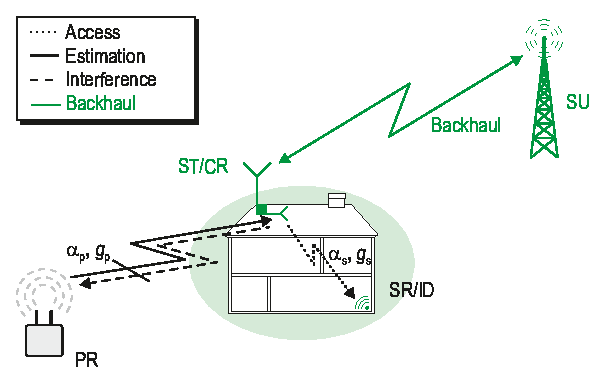
\includegraphics[width=0.55\textwidth]{figures/CR_Scenario_Underlay}%
	}
	\subfloat[]{
	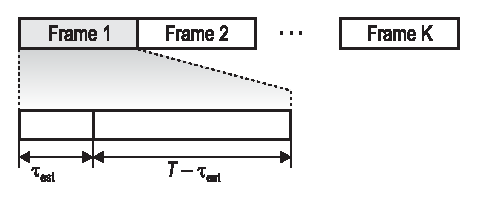
\includegraphics[width=0.45\textwidth]{figures/Frame_Structure_grau_U}%
	}
	\caption{(a) An illustration of a small cell scenarios demonstrating an underlay paradigm. (b) Frame structure at the ST that presents a time duration ($\tau$) allocated within the frame duration for the estimation of the interference channel.} 
	\label{szenarioA}
	%\vspace{-10 pt}
\end{figure}



\figurename~\ref{szenarioA} depicts a small cell deployment consisting of a CSC-BS, a MS, a PR and a MC-BS. Analog to the previous scenarios, the CSC-BS and the MS represent a ST and a SR. The channels between the PR and the ST and between the ST and SR are designated as interference and access channels with channel gains $\gpo$ and $\gs$, respectively. A power control mechanism is employed at the ST to ensure that interference received at the PR is below a certain level. In order to carry out power control mechanism, it is necessary to acquire the knowledge of the channel between the ST and the PR. As proposed in chapter \ref{chap:US}, the ST can retrieve this information by listening to a pilot or beacon signal transmitted by the PR. %For the received pilot signal ($y_\textrm{rcvd}$) and its power, we use the model and notations from \cite{Kaushik15}.


A slotted medium access is implemented at the ST with a frame duration of $T$. The knowledge of the interference channel is acquired by employing channel reciprocity over the link PR-ST. $T$ is designed such that the channel can be assumed to remain constant within it. %Based on this premise, $g_\textrm{p}$ and $g_\textrm{s}$ are constant within one frame and included in $\alpha_\textrm{p}$ and $\alpha_\textrm{s}$ for further analysis.
In order to implement a power control mechanism, the frame interval is divided in two phases, refer to Fig. \ref{szenarioA}. During the estimation phase of duration $\test$ (estimation time), the ST measures the received power of the pilot signal transmitted by the PR. Based on this received power, the ST estimates $\ehpo$ and control its transmit power for the secondary link in order to satisfy the interference constraint at the PR. During the data transmission phase $T-\test$, the ST transmits data with the controlled power to the SR.

\subsection{Signal Model}

%ived signal at the ST, transmitted by the PR cf. \figurename~\ref{fig:scenario}, is sampled with a sampling frequency of $\fsam$ and is given by
\begin{equation}
\yrcvd[n] = \gpo \cdot \xtranpr[n] + \nas[n],
\label{eq:sys_mod_st}
\end{equation}
where $\xtranpr[n]$ corresponds to a discrete constant power signal transmitted by the PR, $\pgpo$ represents the power gain for the channel PR-ST and $\nas[n]$ is circularly symmetric complex Additive White Gaussian Noise (AWGN) at the ST.
The transmitted power at PR is $\ptranpr = \s{\tau \fsam}{|\xtranpr[n]|^2}$, considering that $\tau \fsam$ $(= N)$ is the number of samples used for estimation. $\nas[n]$ is an independent identically distributed (i.i.d.) Gaussian random process with mean $\e{}{\nas[n]} = 0$ and variance $\e{}{|\nas[n]|^2} = \nps$. The estimated received power at the ST is given as
\begin{align}
\prcvd = \s{\tau \fsam}{ |\gpo \xtranpr[n] + \nas|^2}.
\label{eq:prcvd} 
\end{align}
During the data transmission with controlled power at the ST, the received signal at the PR is given by
\begin{equation}
\yp[n] = \gpo \cdot \xscont[n] + \nap[n],
\label{eq:sys_mod_pr}
\end{equation}
and on the other side, the received signal at the SR follows
\begin{equation}
\ys[n] = \gs \cdot \xscont[n] + \nas[n],
\label{eq:sys_mod_sr}
\end{equation}
where $\xscont[n]$ is an i.i.d. random process. The controlled power at the ST is determined as 
\begin{align}
\preg = \s{(T - \tau) \fsam}{|\xscont[n]|^2} 
\label{eq:preg} 
\end{align}
Further, $\pgpo$ and $\pgs$ represent the power gains for channel ST-PR and ST-SR, cf. \figurename~\ref{szenarioA}.
The received powers at the PR and the SR are evaluated as 
\begin{align}
\prcvdpr = \s{(T - \tau) \fsam}{|\yp[n]^2|}  \intertext{ and} \prcvdsr = \s{(T - \tau) \fsam}{|\ys[n]^2|}, 
\end{align}
respectively. Likewise (\ref{eq:sys_mod_st}), $\nap[n]$ and $\nas[n]$ represents circularly symmetric AWGN at PR and ST with zero mean and variance $\e{}{|\nap[n]|^2} = \npp$ and $\e{}{|\nas[n]|^2} = \nps$, correspondingly. %Consider that $\ptran$, $\preg$ and $\pp$ correspond to power for a given frame. 
%For (\ref{eq:sys_mod_sr}), we assume that the interference at SR from the PR via beacon or pilot channel is $< \nps$, which is a valid assumption considering the indoor scenario depicted in \figurename~\ref{fig:scenario}. 
%For (\ref{eq:sys_mod_sr}), we consider a perfect allignment of the ST to the beacon or pilot channe
%\subsubsection{Channel}

Upon utilizing $\tau$ for channel estimation, the throughput at the SR (secondary throughput) over the access channel is given by
\begin{equation}
\rs = \frac{T - \tau}{T} \log_2 \left(1 + \frac{\gs \preg }{\nps} \right). 
\label{eq:sthr}
\end{equation}


All transmitted signals are subjected to distance dependent path loss and small scale fading gains depicted as $\gpo, \gs$. In the analysis, the coherence time of the channels $\approx T$ is considered. But, there will be scenarios where the coherence time exceeds $T$, in such cases the expressions derived in this chapter depicts a lower performance bound.


\section{Theoretical Analysis}
\label{model}
The sequence of events followed by the underlay scenario from Fig. \ref{szenarioA} can be summarized as:

\begin{enumerate}
	%\item The PR sends a pilot signal with power $\ptranpr$ to the ST.
	\item The ST estimates the power received $\eprcvd$ by listening to the pilot signal received from the PR over the interference channel. In the context of the hardware implementation, an unmodulated sinusoidal signal is sent as a pilot or beacon signal\footnote{The sinusoidal signal is mathematically equivalent to the constant power signal sent by the PR, which resembles a constant phase modulated signal or a perfectly downsampled (satisfies Niquist criterion) PSK signal.}.
	\item With the knowledge of the $\ptranpr$ and the estimate $\eprcvd$, the ST indirectly acquires the knowledge of $\epgpo$. 
	Upon acquiring this knowledge, a power control is employed at the ST. Using $\eprcvd$, $\epreg$ is determined as 
\begin{align}
\epreg = \frac{\ite K}{\eprcvd}, \label{eq:preg} 
\end{align}
where $K$ represents a scaling factor. The scaling factor is required at the ST to hold $\e{}{\eprcvdpr}$ at $\ite$. It is defined as
\begin{align}
K = \frac{1}{ \e{\eprcvd}{\frac{\gpo}{\eprcvd}}},% = \fr
\end{align}
where, $\e{\eprcvd}{\cdot}$ represents the expectation over $\eprcvd$.
	%It is scaled such that, in case of perfect channel reciprocity and the absence of noise on the primary link, the interference power arriving at the PR ($\prcvdpr$) has the value of the interference temperature ($\ite$). %In control theory terms, $\ite$ is the setpoint for $\prcvdpr$.
	\item The ST transmits data to the SR with $\preg$. 
	%\item The SR receives the data signal with power $\preg$ It provides this value back over a feedback channel to the ST, where it is used to estimate the expected secondary throughput $\e{\rs}{\rs}$ over the access channel.
	The received power-based estimation ($\eprcvd$) over the interference channel induces variations in controlled power defined as $\epreg$. Following the relation between the controlled power at the ST and the received power at the PR 
\begin{align}
\eprcvdpr  = \hpo \epreg,
\label{eq:eprcvdpr}
\end{align}
the variations in $\epreg$ translate to the variations in $\prcvdpr$ (defined as $\eprcvdpr$) around $\ite$, which result in excessive interference at the PR. Unless captured, these variations may severely degrade the performance of the US. Besides this, due to the relationship between between the controlled power and the secondary throughput defined in (\ref{eq:sthr}), a certain amount of the variations are further translated to the secondary throughput. These variations in the system parameters ($\eprcvd$, $\epreg$, $\eprcvdpr$ and $\ers$) are characterized in terms of their probability density functions (pdfs).  
	\item In particular, the pdf of $\eprcvdpr$ is utilized to employ an interference constraint in terms of confidence probability $\pco$ at the ST such that the excessive interference at the PR can be regulated. In addition, by utilizing the pdf of $\ers$, the performance of the access channel is determined in terms of the expected secondary throughput. Finally, subject to the interference constraint on the confidence probability the performance of the US is jointly characterized in terms of a tradeoff between the estimation time and secondary throughput tradoff. 
\end{enumerate}

\subsection{Characterization of the System Parameters}
In order to capture the variations induced due to channel estimation, the pdfs of the aforementioned system parameters ($\eprcvd$, $\epreg$, $\eprcvdpr$, $\ers$) are characterized, subsequently. 

In accordance to the employed signal model, $\prcvd$ is modeled as a non-central chi-squared distribution $\ncchi2$, whose pdf is characterized as \cite{Char99}
\begin{equation}
	\label{nxc2equ}
	\dprcvd (x) = 
	\frac{N}{2\sigma_\textrm{p}^2} \left(\frac{N x}{\lambda}\right)^\frac{N-2}{4}  
	\exp\left(-\frac{N x+\lambda}{2\sigma_\textrm{p}^2}\right)  I_{\frac{N}{2}-1}\left(\frac{\sqrt{N x\lambda}}{\sigma_\textrm{p}^2}\right) \;  ,
\end{equation}
where $N$ is the degree of freedom and the number of samples used for estimating $\eprcvd$, $\npp$ is the noise variance of the in-phase or quadrature-phase component of the received pilot signal ($\yrcvd[n]$, refer to \ref{eq:sys_mod_st}), and $I_{\frac{N}{2}-1}(\cdot)$ is the modified Bessel function of the first kind of order $\frac{N}{2}-1$ \cite{Jef00}. Furthermore, the non-centrality parameter is defined as
\begin{equation}
	\label{lambda}
	\lambda = \sum_{n=1}^N |\mathbb{E}[|\yrcvd[n]|^2] = N \times A^2
\end{equation}
The simplification in (\ref{lambda}) is explained as follows: a sinusoidal signal that represents a pilot signal consists of a constant amplitude, which is down-converted by an I/Q demodulator at the ST. In this regard, the complex samples $\yrcvd[n]$ have a constant envelope of value $A$. 

Corresponding to (\ref{eq:preg}), $\epreg$ follows an inverse non-central chi-squared distribution. The pdf for $\epreg$  is given by
\begin{align}
\dpreg(x) =& \frac{N K \ite}{2\npp x^2} e^{- \frac{N}{2 \npp}\left( \frac{K  \ite}{x} + \gpo \ptran \right)} \left( \frac{K \ite}{x \gpo \ptran}   \right)^{\frac{N}{4} - \frac{1}{2}} \label{eq:dpreg_pl} \times \\
\quad & I_{\frac{N}{2}  - 1}\left( \frac{N}{\npp} \sqrt{\frac{ K \ite \gpo \ptran}{x}}  \right). \nonumber
%\fpreg(x) = \q{\frac{N}{2} - 1}{\sqrt{\frac{N \ptran \ap}{\npp}},\sqrt{\frac{N \cdot x}{\npp}} }, 
\end{align}
%where $\q{\frac{N}{2} - 1}{\cdot, \cdot}$ is the Marcum-Q function \cite{grad}.
%where $I_{\frac{N}{2}  - 1}(\cdot)$ represents the Bessel function of order $\frac{N}{2} - 1$ \cite{grad}.

Considering the $\dpreg(x)$ defined in (\ref{eq:dpreg_pl}) and the relation described in (\ref{eq:eprcvdpr}), the pdf of $\eprcvdpr$ is determined as 
\begin{align}
\dprcvdpr(x) =& \frac{\ap N K \ite}{2\npp x^2} e^{- \frac{N \ap}{2 \npp}\left( \frac{K  \ite}{x} + \ptran \right)} \left( \frac{K \ite}{x \ptran}   \right)^{\frac{N}{4} - \frac{1}{2}} \times \label{eq:dpp_pl} \\
\quad & I_{\frac{N}{2}  - 1}\left( \frac{N \ap}{\npp} \sqrt{\frac{ K \ite \ptran}{x}}  \right). \nonumber
\end{align}

%The definition of $P_\textrm{c}$ can be retrieved from \cite{Kaushik15}. 
Consequently, the cumulative distribution function (cdf) of $\eprcvdpr$ is given by %\footnote{In \cite{Kaushik15}, we discovered a small typing error in the cdf of $P_\textrm{p}$, in this paper, we present the exact version of it.}
\begin{equation}
	\label{kumu}
	\fprcvdpr = Q_{\frac{N}{2}}\left(\sqrt{\frac{N P_\textrm{tran} \alpha_\textrm{p}}{\sigma_\textrm{p}^2}},\sqrt{\frac{N \alpha_\textrm{p} \theta_\textrm{I} K}{\sigma_\textrm{p}^2 x}}\right) \;  ,
\end{equation}
where $Q_{\frac{N}{2}}(\cdot)$ is the Marcum Q-function \cite{Jef00}.

%The system variables $P_\textrm{cont}$, $P_\textrm{p}$, and $R_\textrm{s}$ are derived from $P_\textrm{rcvd}$ in \cite{Kaushik15}, where the respective pdfs $f_{P_\textrm{cont}}(\cdot)$ and $f_{P_\textrm{p}}(\cdot)$ are also provided. In \cite{Kaushik15}, $f_{R_\textrm{s}}(\cdot)$ represented a pdf of the capacity. Here, we modify this expression to determine the pdf of the secondary throughput
Next, the pdf of the secondary throughput $\rs$ is determined as
\begin{equation}
	\label{Rspdf}
	f_{R_\textrm{s}}\left(x\right) =
	\frac{T}{T-\tau_\textrm{est}}\frac{N K \theta_\textrm{I} \alpha_\textrm{s} \ln{2}}{2 \sigma_\textrm{p}^2 \sigma_\textrm{s}^2} 
	\left(\frac{p\left(x\right)+1}{\left[p\left(x\right)\right]^2} \right)
	e^{-\frac{N}{2 \sigma_\textrm{p}^2} \left(\frac{K \theta_\textrm{I} \alpha_\textrm{s}}{p\left(x\right)\sigma_\textrm{s}^2} + \alpha_\textrm{p} P_\textrm{tran} \right)}
\end{equation}
\begin{equation*}
	\times \left(\frac{K \theta_\textrm{I} \alpha_\textrm{s}}{p\left(x\right) \alpha_\textrm{p} P_\textrm{tran}\sigma_\textrm{s}^2}\right)^{\frac{N}{4}-\frac{1}{2}}
	I_{\frac{N}{2}-1}\left(\frac{N}{\sigma_\textrm{p}^2}\sqrt{\frac{K \theta_\textrm{I} \alpha_\textrm{p} P_\textrm{tran} \alpha_\textrm{s}}{p\left(x\right) \sigma_\textrm{s}^2}}\right) \;  ,
\end{equation*}
\begin{equation*}
\text{with } p\left(x\right) = 2^\frac{Tx}{T-\tau_\textrm{est}}-1 \;  .
\end{equation*} 



From the deployment perspective, it is challenging to determine the noise power at the PR ($\sigma_\textrm{p}^2$), which characterizes the theoretical expressions, accurately. In this regard, an approximate value of $\sigma_\textrm{p}^2$ is determined using the variance of the envelope of $\yrcvd[n]$\footnote{The value of the noise power evaluated during the calibration (that involves no signal transmission) differed from the one determined while performance the measurements for different values of $\snrrcvd$. It is noticed that the latter approach (as presented later in section \ref{ssec:val}) provided a closer fit to the analytical expressions.}

\subsection{Estimation-Throughput Tradeoff}
It is clear that small $\tau$ results in large variations for the $\eprcvdpr$, and subsequently results in the deviation of $\eprcvdpr$ from $\ite$. If not considered, these variations may affect the performance of the US. To capture these variations, an interference constraint defined in terms of a confidence probability $\pco$ and an accuracy $\mu$\footnote{In order to scale the confidence interval relative to $\ite$.} is proposed. In order to restrict the excessive interference due to channel estimation, it is important to restrain $\pco$ above a certain desired level $\pcod$ for a fixed value of $\mu$. In this regard, the interference constraint is defined as
\begin{align}
\pco = \fprcvdpr \left( {(1 + \mu) \ite}\right)  - \fprcvdpr \left({(1 - \mu) \ite} \right) \ge \pcod, \label{eq:pc} 
\end{align}
where $\left( {(1 + \mu) \ite}\right)$ and $\left({(1 - \mu) \ite} \right)$ represent confidence interval around $\ite$. Using (\ref{eq:pc}) and given set of parameters, it is possible to determine $\pco$ for a certain $\mu$. It is worthy to note that $\pco$ depends $\test$, through $\fprcvdpr(x)$. Besides this, $\e{\ers}{\ers}$ is also related to the estimation time. Hence, from the design perspective, it is essential to select the estimation time appropriately such that the ST the maximum secondary throughput is achieved as well as the interference constraint is satisfied. This relationship is characterized as \textit{estimation-throughput tradeoff} is given by 

%Clearly, there exits a tradeoff that involves maximizing the expected throughput at the SR subject to a probability of confidence constraint given by
\begin{align}
\maxi_{\test}  & \text{      } \e{\ers}{\ers(\test)} 
 \label{eq:sys} \\
\text{s.t.} & (\ref{eq:pc}), \nonumber  
\end{align}



\section{Validation}
\label{ssec:val}
This section illustrates the validation of the theoretical expression derived in the previous section. The measurements necessary for the validation is carried out by means of a software defined platform. The experimental setup for acquiring the measurements is presented subsequently. 
 
\subsection{Experimental Setup}

\begin{figure}
	%\vspace{-10 pt}
	\centering
	
\includegraphics[width=0.8\textwidth]{figures/setup}
	\caption{Measurement setup for the validation of the stochastic model, laptop image from \cite{Laptop}}
	\label{messaufbau}
	%\vspace{-10 pt}
\end{figure}


\begin{figure}
        %\vspace{-10 pt}
        \centering
        \subfloat[Signal with oversampling, where the local oscillator is tunned at $\flo = \SI{55}{KHz}$]
	{
		\begin{tikzpicture}[scale=1]
		\node[anchor=south west,inner sep=0] (image) at (0,0)
		{

			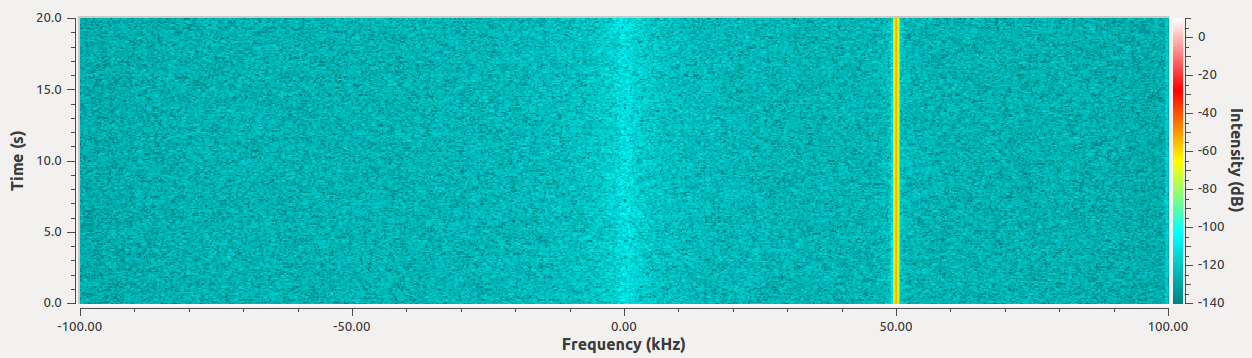
\includegraphics[width=0.9\textwidth]{figures/Spektrum}
        	};
		\begin{scope}[x={(image.south east)},y={(image.north west)}]
		\draw[black,thick,<->] (0.498,0.98) --  node[above, font=\footnotesize] {$\flo = \SI{55}{KHz}$} (0.718,0.98);

		%\draw[help lines,xstep=.1,ystep=.1] (0,0) grid (1,1);
		%\foreach \x in {0,1,...,9} { \node [anchor=north] at (\x/10,0) {0.\x}; }
		%\foreach \y in {0,1,...,9} { \node [anchor=east] at (0,\y/10) {0.\y}; }
		\end{scope}
		\end{tikzpicture}	
		\label{fig:SP_os}
	} \\
        \subfloat[Signal after bandpass filtering, filter bandwidth  $= \SI{50}{KHz}$]
	{

		\begin{tikzpicture}[scale=1]
		\node[anchor=south west,inner sep=0] (image) at (0,0)
		{

			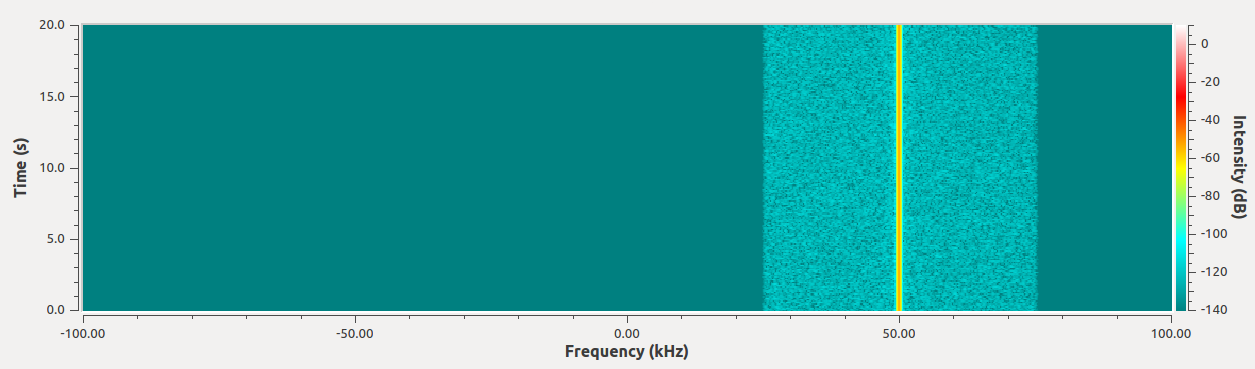
\includegraphics[width=0.9\textwidth]{figures/bpf}
        	};
		\begin{scope}[x={(image.south east)},y={(image.north west)}]
		\draw[black,thick,<->] (0.605,0.98) --  node[above, font=\footnotesize] {Band pass filter = $\SI{50}{KHz}$} (0.825,0.98);

		%\draw[help lines,xstep=.1,ystep=.1] (0,0) grid (1,1);
		%\foreach \x in {0,1,...,9} { \node [anchor=north] at (\x/10,0) {0.\x}; }
		%\foreach \y in {0,1,...,9} { \node [anchor=east] at (0,\y/10) {0.\y}; }
		\end{scope}
		\end{tikzpicture}	
        	\label{fig:SP_bp}
	} \\
        \subfloat[Signal after digital down conversion]
	{
		
\includegraphics[width=0.9\textwidth]{figures/runtergemischt}
        	\label{fig:SP_dc}
	} \\
        \subfloat[Signal after decimation]
	{
		
\includegraphics[width=0.9\textwidth]{figures/dezimiert}
        	\label{fig:SP_de}
	}
        \label{fig:SP}
        %\vspace{-10 pt}
	\caption{An illustration of signal processing carried at the host computer to preclude the spurious effects such as DC Offset and flicker noise, which are significant for signal at low signal to noise ratio.}
\end{figure}


Fig. \ref{messaufbau} presents the experimental setup deployed for performing the validation process. It has been previously claimed that the experimental validation considers the deterministic behaviour of the channel. In this sense, with the employment of the transmit and the receive antennas, the signal received at the at the ST\footnote{The experiments were performed over the ISM bands with center frequency fixed at \SI{2.45}{GHz}, an interference signal from the operational wireless LAN was observed within the band of interest (in-band) or as an out-of-band emissions from the neighbouring channels.} can influence the measurements, thereby resulting in the deviation of the empirical results from their analytical counterpart. To avoid this issue, the interference channel is implemented by means of a coaxial cable. In addition, attenuators are used to realize different values of $\snrrcvd$. %By doing so, we were able to acquire a large number of system variable realizations measured under similar conditions, which we needed for validating the stochastic model. 

The CSC-BS/ST is emulated using a Universal Software Radio Peripherals (USRP) B210, a software defined radio, from Ettus Research \cite{Ettus} and a host computer connected to the USRP by means of USB cable. The host computer performs the following tasks: (i) it enables the access to the USRP by controlling certain RF parameters such as, tunning frequency and sampling frequency, (ii) it allows baseband processing on the complex samples. %Since the characterization of the system parameters, which is associated with the power control is implemented at the ST, therefore it is reasonable to deploy only ST for the validation process. 
The PR is realized using a Rhode $\&$ Schwarz 200A vector signal generator (later for the implementation of the demonstrator, the signal generator emulating the PR is replaced with an USRP and a host computer, like the ST). Since the USRP employs a homodyne receiver\footnote{A homodyne receiver implements a direct down conversion of the bandpass to the baseband signal.}, hence spurious effects arising from the analog front-end can influence the validation process. These spurious effects, particularly, the DC-Offset and the flicker noise around DC become significant at low signal to noise ratio. 

Now, to retrieve the complex samples close to those proposed while deriving the theoretical expressions (which does not take such spurious effects into account), following signal processing is proposed at the host computer. 
\begin{itemize}
\item The received signal is oversampled (with sampling frequency $200$ $\SI{}{KHz}$, for a bandpass filter with bandpass frequency of $\SI{50}{KHz}$ applied subsequently, this sampling corresponds to a oversampling factor = 4) and the local oscillator is tunned at a certain offset frequency defined as $\flo = \SI{50}{KHz}$, refer to \figurename~\ref{fig:SP_os}. 
\item Subsequently, a bandpass filter (with bandwidth = $\SI{50}{KHz}$) is employed to obtain the desired bandpass signal at the $\flo$, which filters out the DC-Offset and the flicker noise present at low frequencies, cf. \figurename~\ref{fig:SP_bp}. 
\item In order to obtain the low pass equivalent of the desired signal, a digital down conversion\footnote{Multiplying with a complex sinusoid with frequency $\flo$.} over the bandpass filtered signal is performed, cf. \figurename~\ref{fig:SP_dc}. %These four steps depicted in \figurename~\ref{fig:SP} are carried out to remove the receiver's DC offset and the flicker noise (1/f) around the DC. Due to the small bandwidth of the pilot signal, these effects form the bottleneck of our validation and had to be accounted for. 
\item In the end, decimation (refer to \figurename~\ref{fig:SP_de}) of the oversampled down converted signal is performed to reduce the correlation between the samples due to oversampling, since the proposed framework considers independent and identically distributed samples for characterizing the pdfs of the corresponding systems parameters. 
\end{itemize}
To complement the validation process, the measurement data is analyzed offline using Matlab.


\subsection{Validation of System Parameters}

Since the stochastic model is the basis of the performance analysis of the proposed framework. It is reasonable to first validate the pdfs of the system variables $\eprcvd$, $\epreg$, $\eprcvdpr$, and $\ers$ derived in Section \ref{model}. To this end, measurements with the setup in Fig. \ref{messaufbau} have been performed for different values of received signal-to-noise ratio at the ST over the interference channel link ($\snrrcvd$\footnote{As noise power, the measured receiver noise floor.}). The measurement data was plotted in terms of histograms and scaled such that it represented the relative frequency ($f_\textrm{rel}$). Fig. \ref{hrel_pdf} compares the histograms from the measurements and plotted pdfs using the analytical expressions for different system parameters. The plots show that the theoretical expressions very accurately capture the performance of the CR systems operating under realistic situations.



\begin{figure}
	%\vspace{-10 pt}
	\centering
	\includegraphics[width=0.5\textwidth]{figures/40}%
	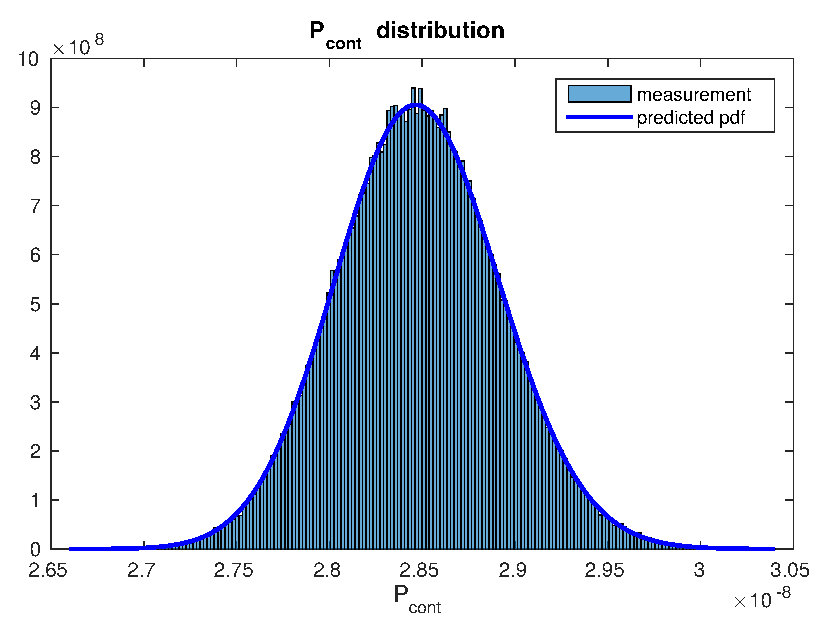
\includegraphics[width=0.5\textwidth]{figures/P_cont_40dBm_k100}%
	
	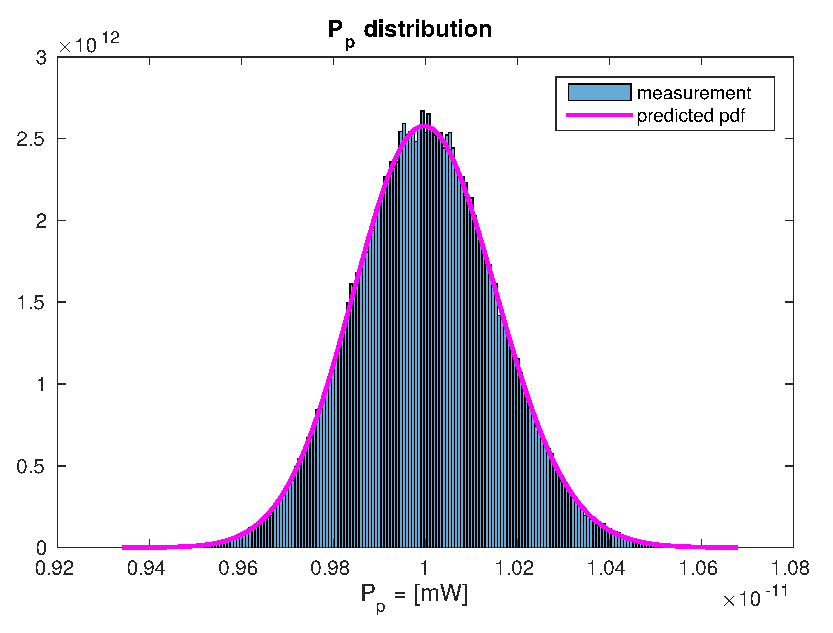
\includegraphics[width=0.5\textwidth]{figures/P_p_40dBm_k100}%
	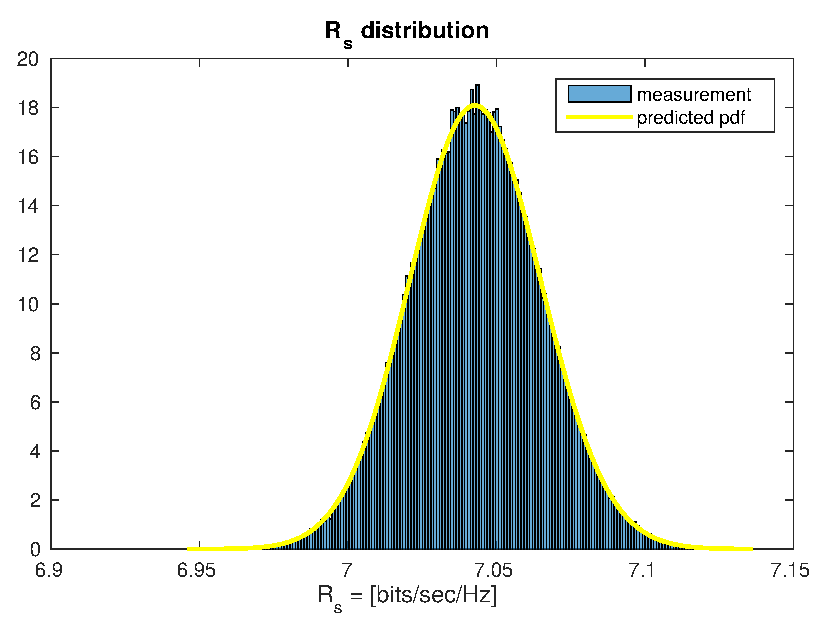
\includegraphics[width=0.5\textwidth]{figures/R_s_40dBm_k100}%
	\caption{Theoretical expressions of the pdf and experimental results of different system variables (parameters from Table \ref{param})}
	\label{hrel_pdf}
	%\vspace{-10 pt}
\end{figure}

The experiments were repeated for different values of $\snrrcvd$. It was observed that for a considerable range of $\snrrcvd \in (4,30)\SI{}{dB}$, the theoretical expressions depicted a significant accuracy to the experimental data, refer to Table \ref{nichtzentral}. The accuracy was quantified in terms of relative error ($e_\textrm{rel}$) defined as
\begin{equation}
\label{fr}
e_\textrm{rel} = \frac{1}{|\mathcal X\sub{bins}|} \times \sum_{x \in \mathcal X\sub{bins}} \frac{\dprcvd(x) - f\sub{hist}[x]}{f\sub{hist}[x]} \;  , 
\end{equation}
where $f\sub{hist}(x)$ corresponds to a histogram evaluated over a set of bins $\mathcal X\sub{bib}$. $|\mathcal X\sub{bins}|$ represents the cardinality of $\mathcal X\sub{bins}$, which excludes bins with $f\sub{hist}[x] \neq 0$. 

\begin{table}
%	\vspace{-10 pt}
	%\setlength{\tabcolsep}{6pt} % spacing between columns
	\renewcommand{\arraystretch}{1.4}
	\centering
	\caption{Values of the parameters used for the performing experiments.}
	\label{param}
	\begin{tabular}{c||c}
		\bfseries Parameter & \bfseries Value \\ \hline \hline
		$\snrrcvd$ & \SI{22}{dB} \\
		$N$ & 100 \\
		$\test$ & \SI{0.5}{ms}\\
		$\ite$ & \SI{-110}{dBm}\\
		$T$ & \SI{100}{ms}\\
		$\pgs$ & 1 \\
		$\npp$ & $2.1355\times10^{-10}$\\ \hline
		%Value & \SI{22}{dB} & 100/\SI{0.5}{ms} & \SI{-110}{dBm} & \SI{100]{ms} & 1 \tablefootnote{The channel gain of the ST-SR link $\alpha_\textrm{s} \in (0,1)$ was set to its maximum theoretical value for this analysis.} & $2.1355\times10^{-10}$ \tablefootnote{The value represents the measured receiver noise floor (digital value) of the in-phase or quadrature-phase components.} \\ 
	\end{tabular}
%	%\vspace{-10 pt} 
\end{table}

\begin{table}
%	%\vspace{-10 pt}
	%\setlength{\tabcolsep}{3pt} % spacing between columns
        \renewcommand{\arraystretch}{1.4}
	\centering
	\caption{$e\sub{rel}$ for different values of $\snrrcvd$}
	\label{nichtzentral}
	\begin{tabular}{c||c} 
		\bfseries $\snrrcvd$/[dB] &  \bfseries $e_\textrm{rel}$ \\ \hline \hline
		$4.08$ &  $0.0568$ \\
		$9.10$ &  $0.0601$ \\
		$14.11$ & $0.0522$ \\
		$19.12$ & $0.0437$ \\
		$24.09$ & $0.0506$ \\
		$29.09$ & $0.0634$ \\
		$34.03$ & $0.1179$ \\
		$39.38$ & $0.0800$ \\
		$45.08$ & $0.1695$ \\ \hline
		%$e_\textrm{rel}$ & $0.0568$ & $0.0601$ & $0.0522$ & $0.0437$ &	$0.0506$ & $0.0634$ & $0.1179$ & $0.0800$ & $0.1695$ \\ 
	\end{tabular}
%	\vspace{-10 pt} 
\end{table}


\subsection{Validation of the Estimation-Throughput Tradeoff}

Here, the performance in terms of estimation-throughput tradeoff is validated, that yields a suitable estimation time that satisfies the interference constraint on $\pco$ and maximizes the achievable throughput. In contrast to the theoretical analysis presented in Fig. \ref{RspocstricheA}, an empirical validation to the performance of the underlay system is provided. As discussed previously, this tradeoff illustrates that a large $\test$ improves the performance of the primary system by reducing the variations in $\eprcvdpr$, depicted in terms of an increase in $\pco$. From the perspective of the secondary system, the increase in $\test$ reduces the achievable secondary throughput.
\begin{figure}
	%\vspace{-10 pt}
	\centering
	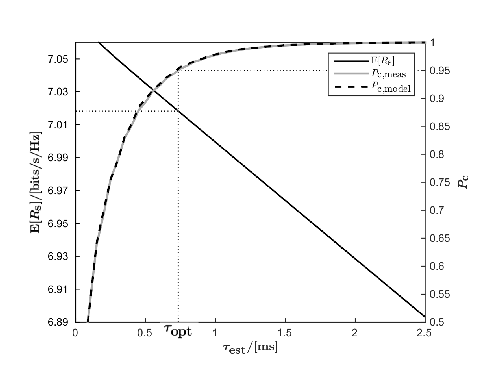
\includegraphics[width=0.8\textwidth]{figures/Rs_poc_striche}
	\caption{Estimation-throughput tradeoff (parameters from Table \ref{param}), $P_\textrm{c,meas}$: empirical values of $P_\textrm{c}$, $P_\textrm{c,model}$: analytical values of $P_\textrm{c}$.}
	\label{RspocstricheA}
	%\vspace{-10 pt}
\end{figure}
Fig. \ref{RspocstricheA} presents the joint validation of the performance parameter $\pco$ and $\e{\ers}{\ers}$. This is achieved by comparing its empirical values with its analytical expressions for different $\test$. In contrast to the analytical framework presented in Section \ref{model}, the empirical values of $\pco$ were determined by computing a numerical integration in the region within the confidence interval $(1  \pm \mu)  \theta_\textrm{I}$. Hence, with this verification, it is concluded that the received power based-technique and consequently the analytical framework proposed for determining the performance of the US is suitable for hardware implementation.

\section{Implementation of a Demonstrator}
\label{demo}
Upon validating the proposed approach, which considers the offline verification of the proposed approach. From the deployment perspective, it is interesting to demonstrate the online operation of the underlay paradigm on a real hardware. This section provides insights and outline the involved issues while deploying the proposed approach by means of a demonstrator. 

\subsection{Estimation Time}
\label{esttime}
The analytical expression in (\ref{eq:sys}) and illustrated in Fig. \ref{RspocstricheA}) depicts a dependency of the performance parameters ($\pco$ and $\e{\ers}{\ers}$) on the estimation time $\test$. This dependency (depicted as estimation-throughput tradeoff) is utilized to determine the suitable estimation time $\ttest$ that achieves the maximum secondary throughput. However, $\ttest$ can be determined for a certain value of the $\snrrcvd$ (for a given channel gain). In practice, the mobility of the ST or the PR, or the surroundings objectes can affect the channel gain, and consequently the received $\snrrcvd$. Under this situation, it is challenging to select $\ttest$ such that the system adheres to the interference constraints at the PR and still achieves the maximum secondary throughput for the corresponding values of $\snrrcvd$. To approach this issue, the variation of $\ttest$ for a certain range of $\snrrcvd$ and different values of the confidence probability constraint $\pcod \in \{0.90, 0.95, 0.99\}$ is investigated\footnote{Such investigations can be performed during the validation process, which is normally included at the system design.}, cf. \figurename~\ref{fig:Tausnr}. %a new parameter called the estimation time ($\testo$) is introduced. It is $\test$ that maximizes the secondary throughput according to (\ref{eq:}) in \cite{Kaushik15} for a certain value of $\snrrcvd$, $\mu$ and a target value of $P_\textrm{c}$ defined as $\bar{P_\textrm{c}}$. In Fig. \ref{RspocstricheA}, this optimization process is indicated graphically by the dotted lines, where, from a fixed $\bar{P_\textrm{c}} = 0.95$, we acquire $\tau_\textrm{opt} \approx \SI{0.75}{ms}$, which corresponds to $\mathbb{E}\left[R_\textrm{s}\right] \approx \SI{7.02}{bits/s/Hz}$.

%However, this analysis is carried out for a fixed value of $\snrrcvd$. Under real conditions, due to channel fading, $\snrrcvd$ is not known. In this sense, it is not possible to determine $\tau_\textrm{opt}$. To resolve this issue, we propose a procedure, whereby we analyze the variations of $\tau_\textrm{opt}$ for different values of $\snrrcvd$, refer to Fig. \ref{Tausnr}, and select $\tau_\textrm{opt}$'s maximum value. 
Based on this analysis, the maximum value of the suitable estimation time $\ttesto = \maxi\{ \ttest | \snrrcvd \in \{-20,20 \}\SI{}{dB} \}$ is selected as the estimation time for the demonstrator.  
By doing this, it is assured that the interference constraint is satisfied for different realizations of the channel gain, which correspond to $\snrrcvd \in \{-20,20\}\SI{}{dB}$. 
%In addition, we consider different values of $\bar{P_\textrm{c}}$. 
\begin{figure}
	%\vspace{-10 pt}
	\centering
	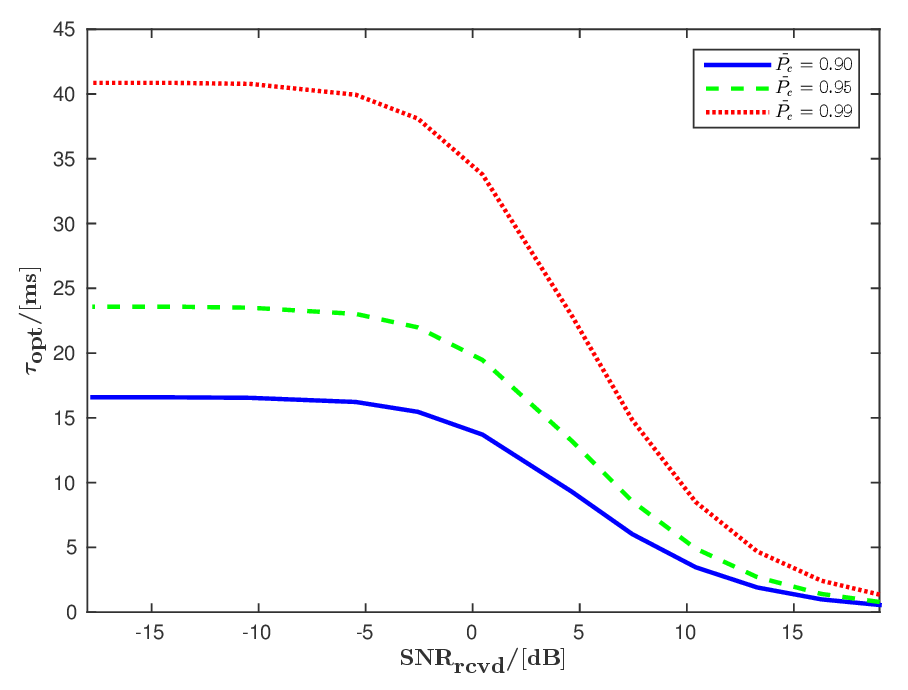
\includegraphics[width=0.85\textwidth]{figures/tau_snr}
	\caption{$\tau_\textrm{opt}$ over $\snrrcvd$, $\theta_\textrm{I}$ = \SI{-110}{dBm}, $\mu$ = 0.05}
	\label{fig:Tausnr}
	%\vspace{-10 pt}
\end{figure}
From \figurename~\ref{fig:Tausnr}, it is further observed that $\ttest$ decreases with $\snrrcvd$ and attains saturation below a certain $\snrrcvd$. %\footnote{For varying $\theta_\textrm{I}$, while the shape of the curves changed slightly, the upper limits for $\tau_\textrm{opt}$ remained constant.} 
This behaviour can be explained as follows: For large values of $\snrrcvd$, $\preg$ is low, hence reduces the variations of $\eprcvdpr$ around $\ite$ and consequently a lower value of $\ttest$ is needed to maintain these variations within the confidence interval. On the other hand, the signals received with low $\snrrcvd$ at the URSP, which correspond to a higher $\preg$, however, considering the limited number of samples used for the estimation process and sensitivity of the hardware, it is difficult to distinguish such signals from the noise. This is why, $\test$ saturates of the $\tau_\textrm{opt}$ below a certain $\snrrcvd$, the received. Upon improving the number of samples or the hardware sensitivity, it is possible to extend the saturation region to the lower $\snrrcvd$. 

In the end, this analysis can be used for determining $\ttesto$ in the implementation of our demonstrator. Since the confidence probability constraint $\pcod = 0.95$ is targeted, $\tau_\textrm{est} = \SI{24}{ms}$ is chosen to be estimation time for the channel estimation, cf. \figurename~\ref{fig:Tausnr}. With this, the interference constraints at the PR is satisfied for all $\snrrcvd$ at the cost of a decreased performance in expected secondary throughput, particularly for the situations with high $\snrrcvd$ that achieves the suitable estimation time at lower value.


\subsection{Simplifications}
\label{ssec:simp2}
In addition to the simplifications proposed for the hardware validation in section \ref{ssec:simp2}, following simplifications are considered for the deployment of the demonstrator: 
%The main objective of this section is to demonstrate the basic principle of an underlay scenario, in view of this, the following reasonable simplifications in the proposed analytical framework is considered:

\begin{enumerate}
	%\item The hardware implementation of the SR is not considered, that is, it is regarded virtual in the system (refer to Fig. \ref{demo_blockA}).
	\item According the proposed framework the controlled power can be evaluated using (\ref{eq:preg}). However, it requires knowledge of the scaling parameter $K$, which further requires the computation of the expected received power $\e{\eprcvd}{\eprcvd}$. However, it is difficult to carry out such computation in practical situations. To deal with this issue, the demonstrator is deployed to evaluate the control power based on a single realization of the $\eprcvd$. This increases the variation in the system. Considering this simplification, it is expected to notice a certain deviation in the performance depicted by the demonstrator to the one depicted by the theoretical expressions. Still for the preliminary deployment, it will be interesting to observe the impact of this simplification on the performance of the demonstrator in terms of the violation of the interference constraint. In this regard, the estimated channel gain, evaluated from $\eprcvd$, is determined as 
	\begin{equation}
		\epgpo = \frac{\e{\eprcvd}{\eprcvd}-\npp}{\ptran} \approx \frac{\eprcvd-\npp}{\ptran}. 
		\label{eq:approx1}
	\end{equation}	
As $\npp$ is negligible compared to $\eprcvd$, (\ref{eq:approx1}) can be further simplified
	\begin{equation}
		\epgpo = \frac{\eprcvd-\npp}{\ptran} \approx \frac{\eprcvd}{\ptran}.
		\label{eq:approx2}
	\end{equation}	
	\item Furthermore, the analytical framework assumes the frame synchronization (in case of Time Division Duplexing) between the PR and the ST. Since, it involves the synchronization of (possibly) two different systems.  which again is complicated to . To simplify this matter, we propose Frequency Division Duplexing between the PR and the ST: We transmit and receive the signals using two different frequencies (\SI{2.422}{GHz} and \SI{2.423}{GHz}) over two separate antennas, as illustrated in Fig. \ref{demo_blockA}. With this technique, the channel reciprocity may be compromised.	
\end{enumerate}

\begin{figure}
	%\vspace{-10 pt}
	\centering
	\includegraphics[width=0.9\textwidth]{figures/demo_block}
	\caption{Setup and block diagram of demonstrator}
	\label{demo_blockA}
	%\vspace{-10 pt}
\end{figure}

Mapping the steps described in Section \ref{scenario} onto hardware and applying the above-mentioned simplifications, we acquire the signal flow illustrated in Fig. \ref{demo_blockA}, which we have implemented in GNU Radio using the available blocks therein.


\subsection{User Interaction and Observations}

Fig. \ref{interface} shows the user interfaces of the demonstrator, providing insights to the parameters evaluated at the PR (for instance, $P_\textrm{p}$ and $P_\textrm{c}$) and the CR/ST (for instance, $P_\textrm{rcvd}$, $P_\textrm{cont}$, and $R_\textrm{s}$). We have performed hardware calibration in the demonstrator to provide physical significance to the digital values obtained from the USRPs, hence the displayed units. As the SR has not been implemented in the hardware, to incorporate the effect of $\alpha_\textrm{s}$ on the performance of the system, we employ a slider to modify its value. %$R_\textrm{s}$ is affected by changing the value of $\alpha_\textrm{s}$ or $T$. 

As expected, changing the value of $\theta_\textrm{I}$ at the CR/ST changes the measured value of $P_\textrm{p}$ at the PR to approximately the same value. This phenomenon is highlighted in Fig. \ref{interface}. At the same time, the values of $R_\textrm{s}$ and $P_\textrm{cont}$ adapt accordingly. This demonstrates that the received power estimation done at the ST by listening to the pilot based channel, thereby acquiring the channel knowledge and performing the power control, is working in accordance to the underlay principle. 

The response to the dynamic conditions can be verified by changing the distance between the PR and ST, the effect can be captured by observing the changes in $P_\textrm{rcvd}$ and other parameters depending on it. As the distance is increased beyond a certain value, the ST operates at its maximum transmit power. This event is indicated in the user interface.

\begin{figure}
	%\vspace{-10 pt}
	\centering
	\subfloat[]
	{
		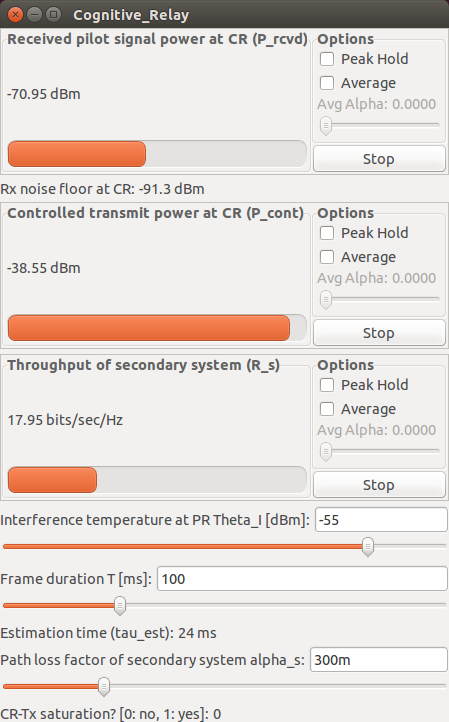
\includegraphics[width=0.5\textwidth]{figures/crinterface}
	}
	\subfloat[]{
	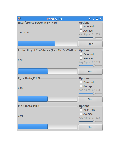
\includegraphics[width=0.5\textwidth]{figures/printerface}
	}
	\caption{A snapshot of the performance parameters displayed in the graphical user interface}
	\label{interface}
	%\vspace{-10 pt}
\end{figure}

With $\mu = 0.05$, the demonstrator does not provide the target value of 0.95 for $P_\textrm{c}$, as the variations in $P_\textrm{p}$ are higher as expected. Certainly, this issue is partly caused by the simplifications undertaken in \ref{alphapschlange}, which have to be accounted for in future implementations. Another possible reason for this observation is that we used a pilot signal produced by a signal generator in the previous analysis, which offers a higher signal quality than the one produced by a USRP in the demonstrator. Moreover, because of the separate links for sensing and transmission and the frequency separation of \SI{1}{MHz}, the channel reciprocity in our demonstrator may be compromised compared with the theoretical model. To resolve this issue, we increase the tolerance limit to $\mu = 0.20$, which leads to the desired $P_\textrm{c}$ of 0.95. On this account, we will consider the signals being transmitted by a USRP for validation, in the future. Despite this, we have been able to demonstrate the principle working of an underlay system that employs a power control mechanism at the ST to limit the excessive interference at the PR.


\section{Summary}
\label{con}

In this paper, we have analyzed the performance of an underlay system from a deployment perspective. To this end, an existing analytical framework \cite{Kaushik15} has been validated. In this regard, the validation of a stochastic model that incorporates the pdfs of the system parameters has been considered. In addition, the performance analysis in terms of estimation-throughput tradeoff has been validated. Based on this validation, it has been illustrated that the proposed framework is suitable for real world deployments. Upon the experimental analysis, a hardware demonstrator that depicts the principle working of the underlay system has been proposed. More importantly, the hardware challenges and simplifications considered while deploying the demonstrator have been briefly discussed.  

In the future, we intend to reconsider certain simplifications made while deploying the demonstrator, for instance, we propose to deploy a USRP for the SR and try to synchronize the frame structure at the ST and the PR in order to respect channel reciprocity.












%Implementation using software defined radio.
%\section{Interweave system}
%
%\subsection{System model}
%
%\subsection{Measurement setup}
%\begin{figure}[!t]
%        \centering
%        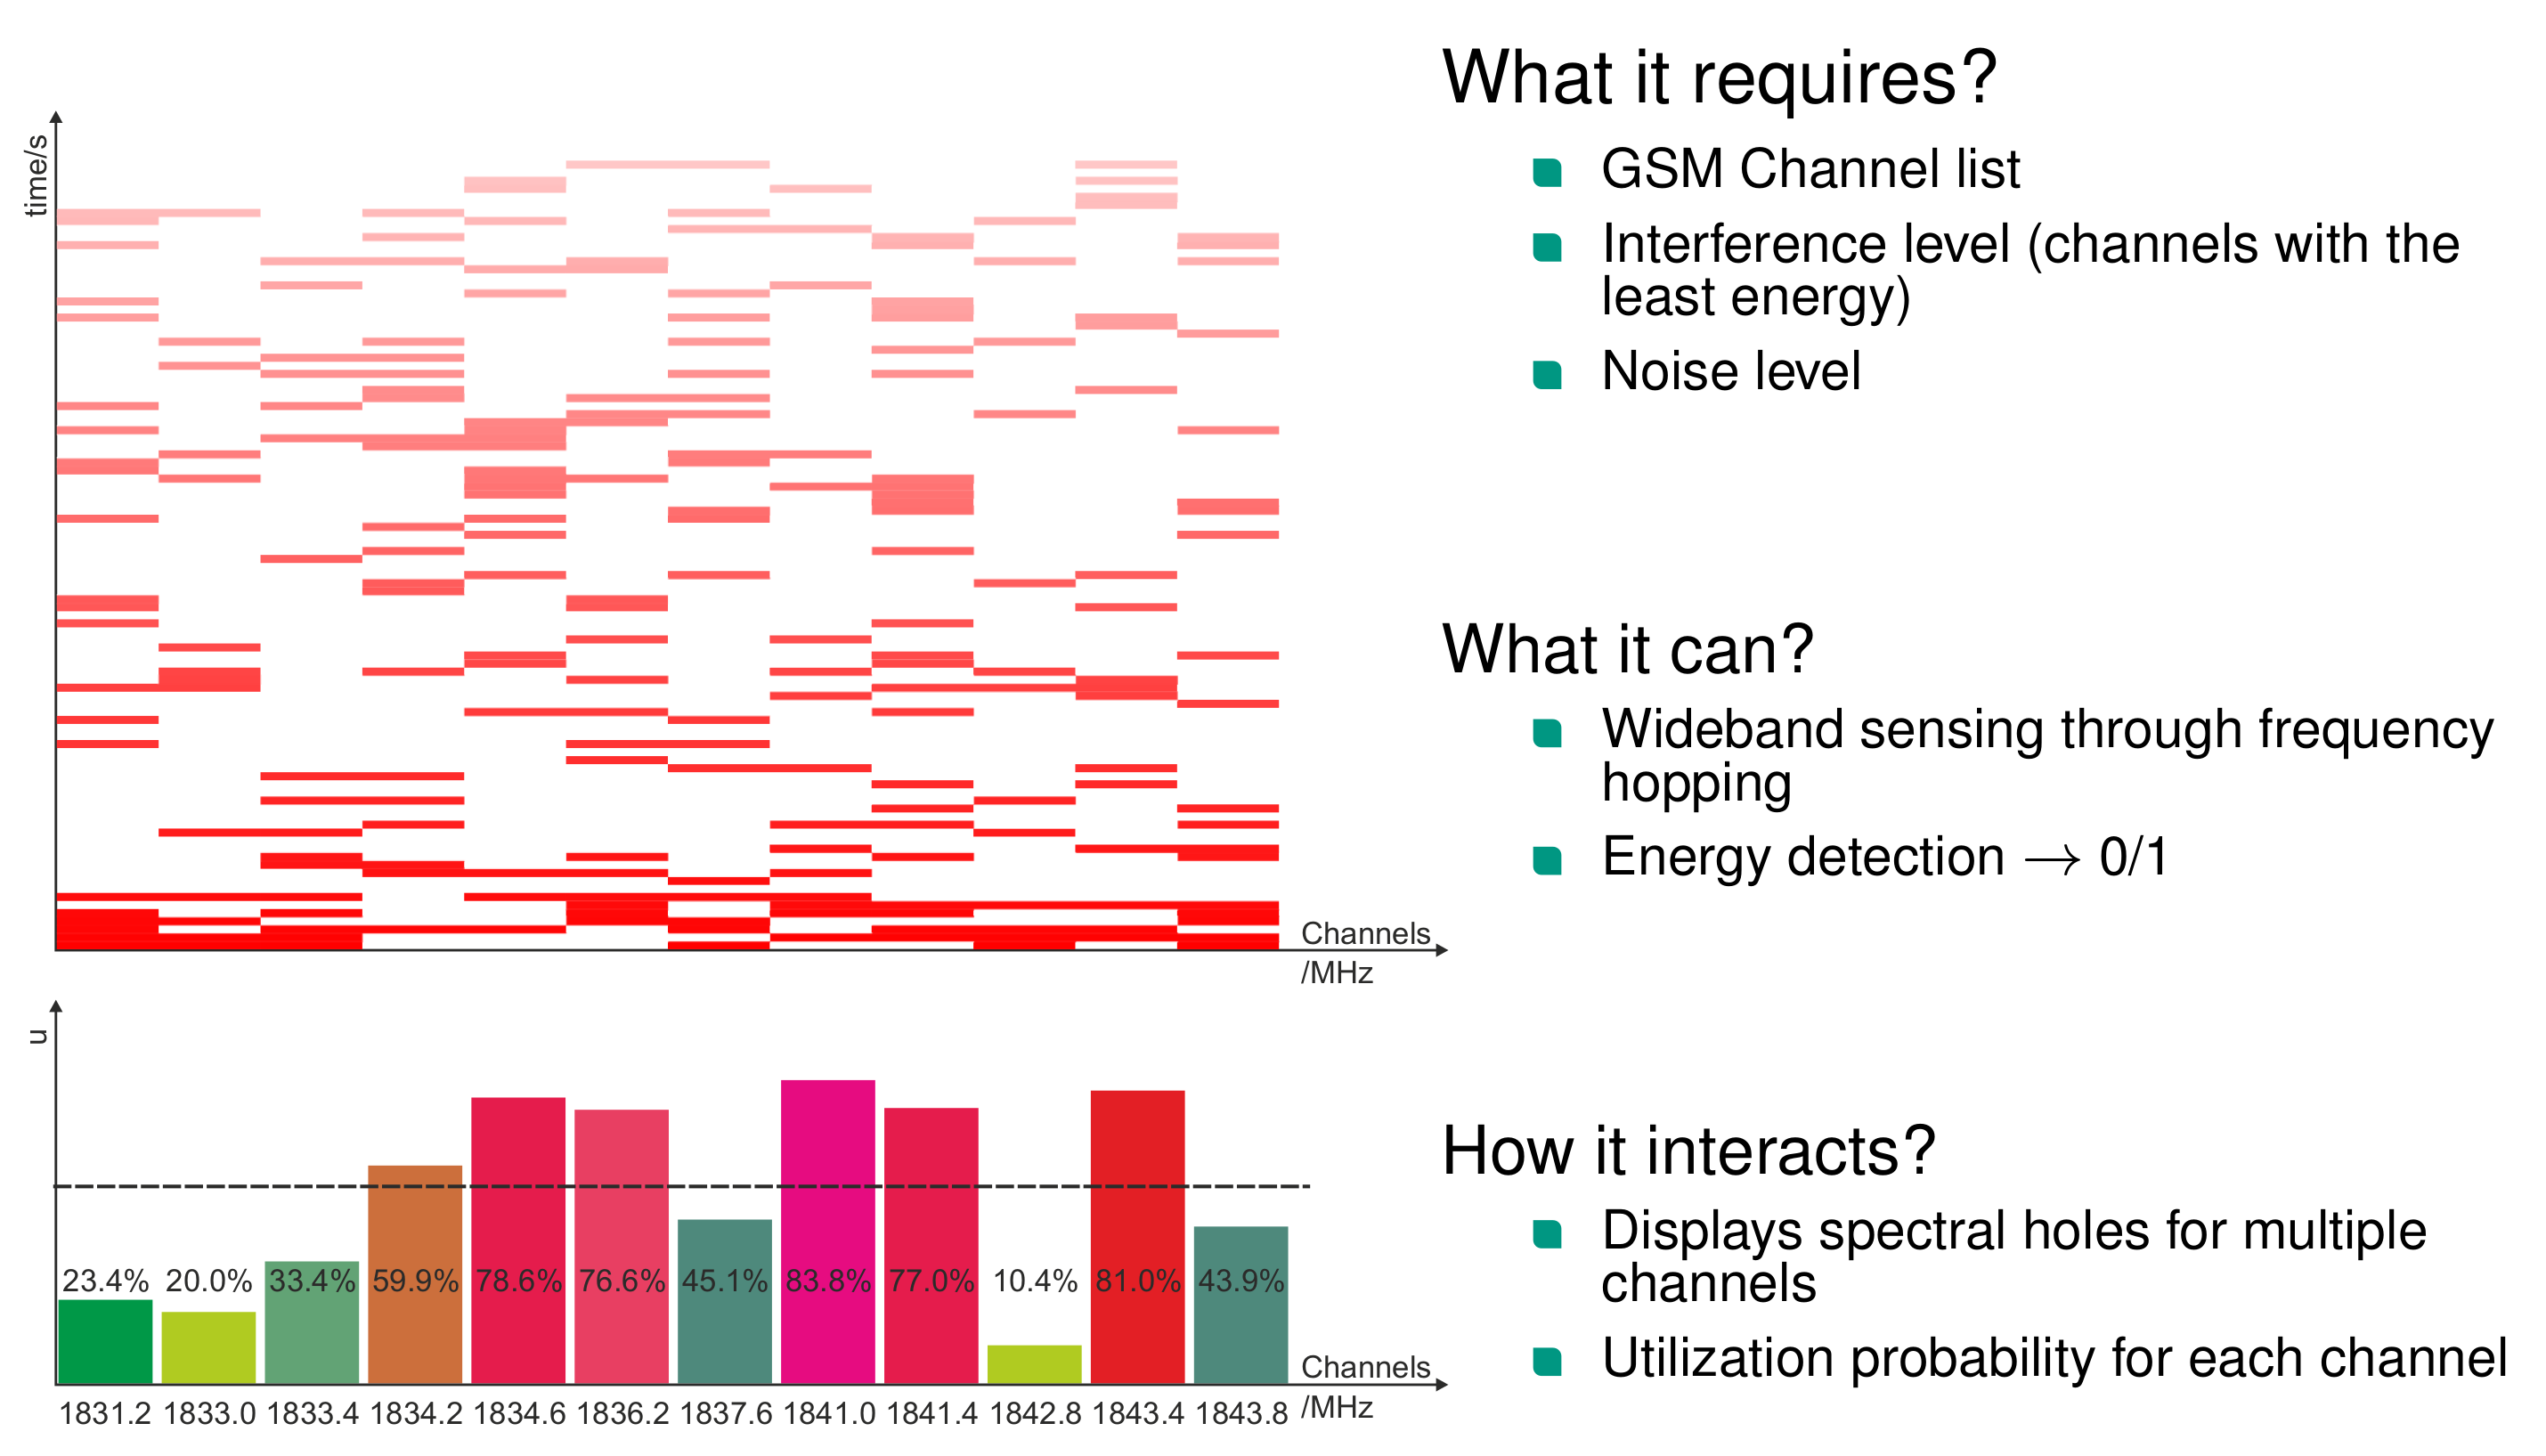
\includegraphics[trim=0.0cm 0.0cm 5.28cm 0.0cm,clip=true,width=\columnwidth]{../kapitel05/figures/Interweave_GUI.png}
%        \caption{Utilization probability for ranking the GSM subchannels.}
%        \label{fig:uti}
%\end{figure}
%Hardware demonstration \cite{Kaushik_ISWCS} of \ac{CR} that
%\begin{itemize}
%\item detects spectrum holes or temporal opportunities in \ac{PU} system 
%\item illustrates cognitive sensing ,i.e, it estimates the spectral occupancy for the multi-band \ac{PU} system
%\end{itemize}
%
%\subsection{Analysis}
%
%\section{Underlay system}
%
%\subsection{System model}
%CR models the channel coefficients $h_\text{p}$, $h_\text{s}$, using Rayleigh or Nakagami-$m$ distribution for the indoor-indoor and indoor-outdoor links. In literature, Rayleigh distribution is mostly preferred due to its analytical tractability. In contrast to that, Nakagami-$m$ accounts for the severity in fading through $m$ parameter, thus, it is more applicable in indoor scenarios. For a fixed transmit power at CR, the received signal to noise power $\gamma$\footnote{Consider a transmission from a certain CR, then $\gamma$ is equivalent to signal to noise ratio (SNR) at ID and interference to noise ratio at PR. Therefore, the term SNR is not used to avoid confusion thereof. Moreover, the interference from unintended primary transmitters and other CRs at PR or ID is treated as white noise.} at PR or ID, corresponding to Rayleigh case, follows exponential distribution \cite{simon2005}
%\begin{equation}
%\label{eq:expo}
%F_{\gamma}(\gamma) = 1 - e^{- \frac{\gamma}{\bar{\gamma}} }
%\end{equation}
%and for Nakagami-$m$, it follows Gamma distribution \cite{simon2005}
%\begin{equation}
%\label{eq:gamma}
%F_{\gamma}(\gamma) = 1 - \frac{ \Gamma{ \left( m, m \frac{\gamma}{\bar{\gamma}} \right) }}{\Gamma(m)},
%\end{equation}
%where $\bar{\gamma} = \mathbb{E}[\gamma]$ and $m$ denotes the shape parameter. $\Gamma(\cdot)$ and $\Gamma(\cdot,\cdot)$ are the complete and incomplete Gamma functions. 
%
%
%\begin{figure}[!t]
%        \centering
%        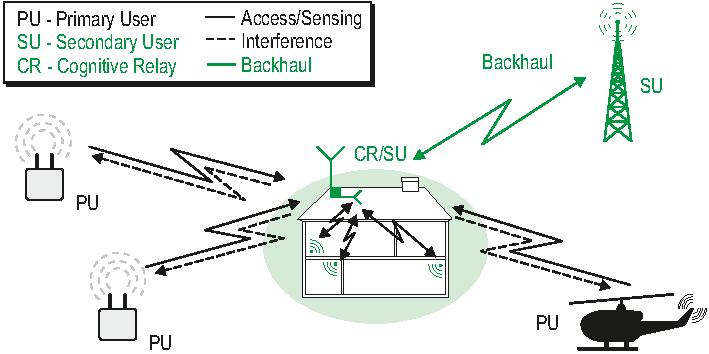
\includegraphics[width = \columnwidth]{../kapitel05/figures/wo_channels_CR_Scenario_farbig_general}
%        \caption{A scenario demonstrating the interaction between the PU and the CR. The CR senses PUs channels in the outdoor to provide a dynamic access to the devices operating indoor.}
%        \label{fig:scenario}
%\end{figure}
%
%\begin{figure}[!t]
%        \centering
%        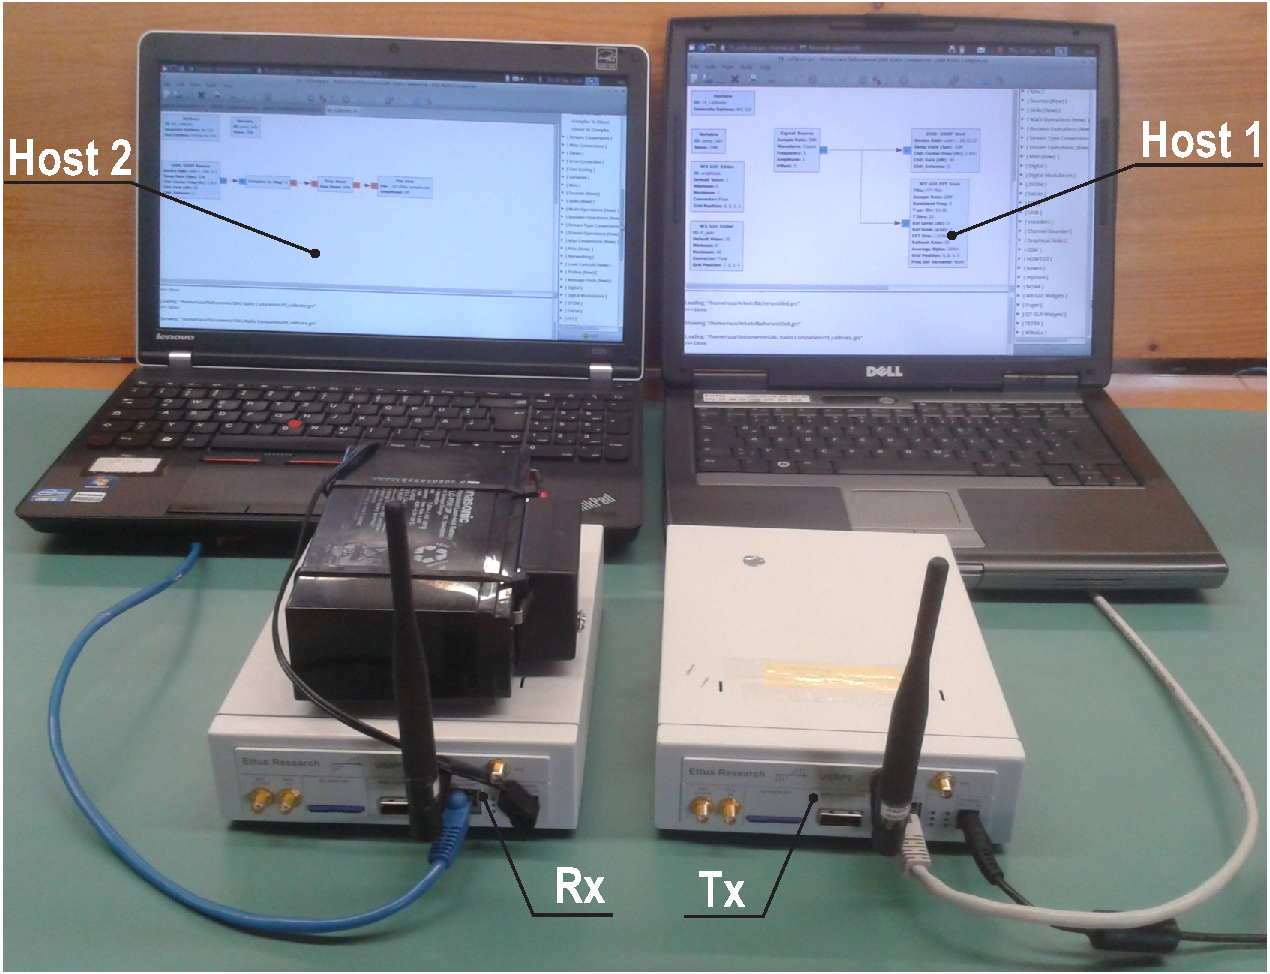
\includegraphics[width = 0.8\columnwidth]{../kapitel05/figures/setup}
%        \caption{Hardware setup.}
%        \label{fig:hw_setup}
%\end{figure}
%
%
%\ac{CR} operating as underlay system \cite{Kaushik_CROWNCOM}
%\begin{itemize}
%\item deploys propagation models to capture movements of \ac{PR} and \ac{ID}
%\item implements sharing constraints to access the \ac{PU} channel 
%\end{itemize}
%
%\subsection{Measurement setup}
%\begin{figure}[!t]
%        \centering
%        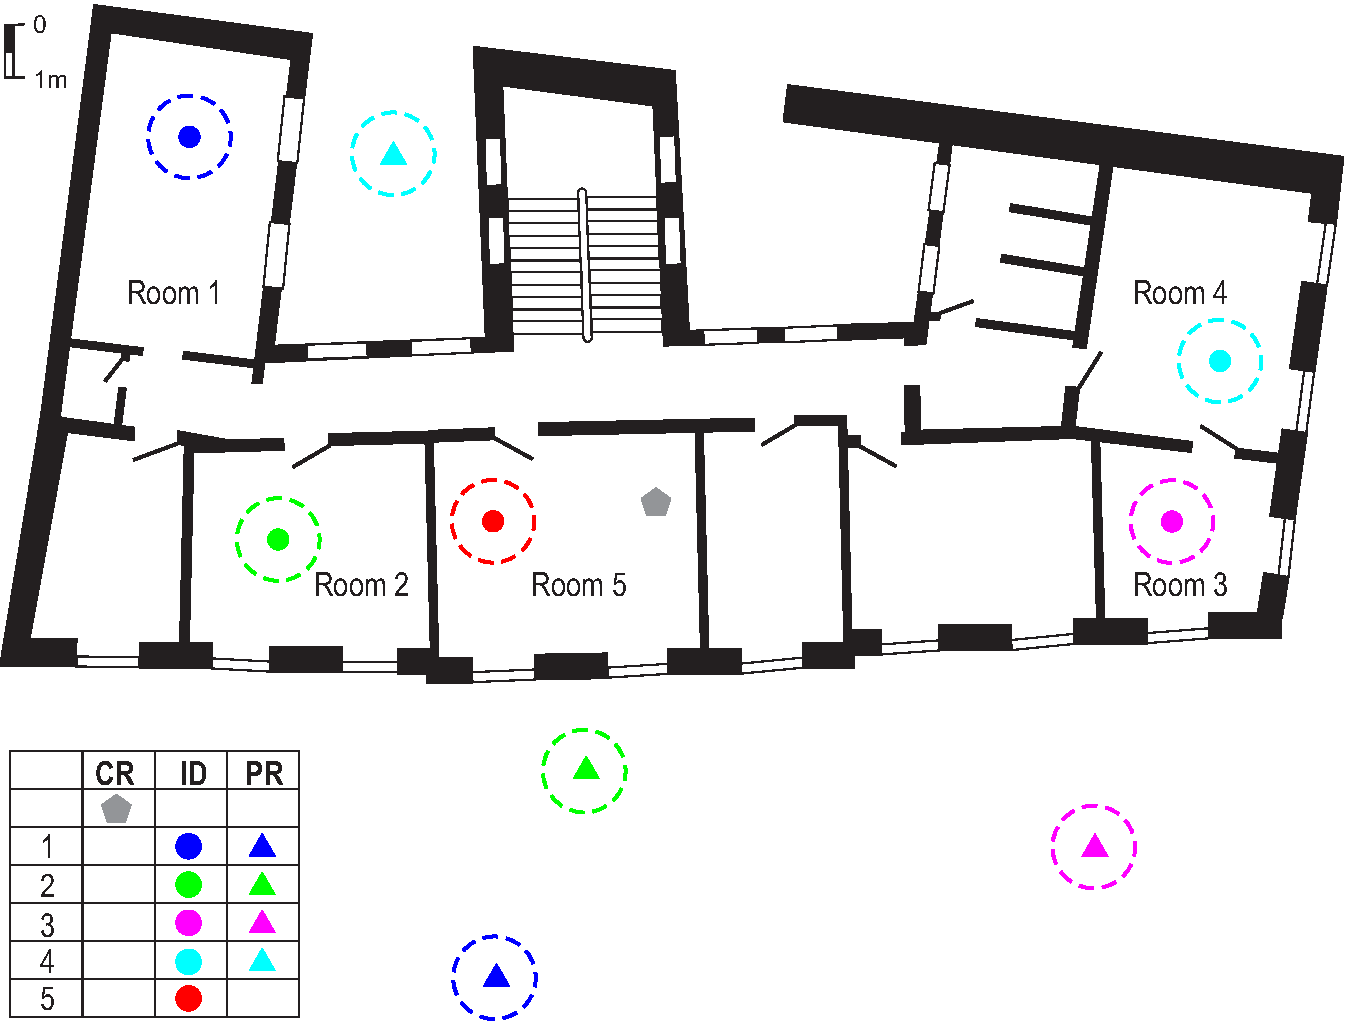
\includegraphics[width = \columnwidth]{../kapitel05/figures/floor_B}
%        \caption{The deployment scenario for the CR including ID and PR at different spatial positions. The circle around the PR and ID positions represents $\mathbb{R}$, which illustrates their small movements.}
%        \label{fig:deploymentScenario}
%\end{figure}
%
%\begin{figure}[!t]
%        \centering
%        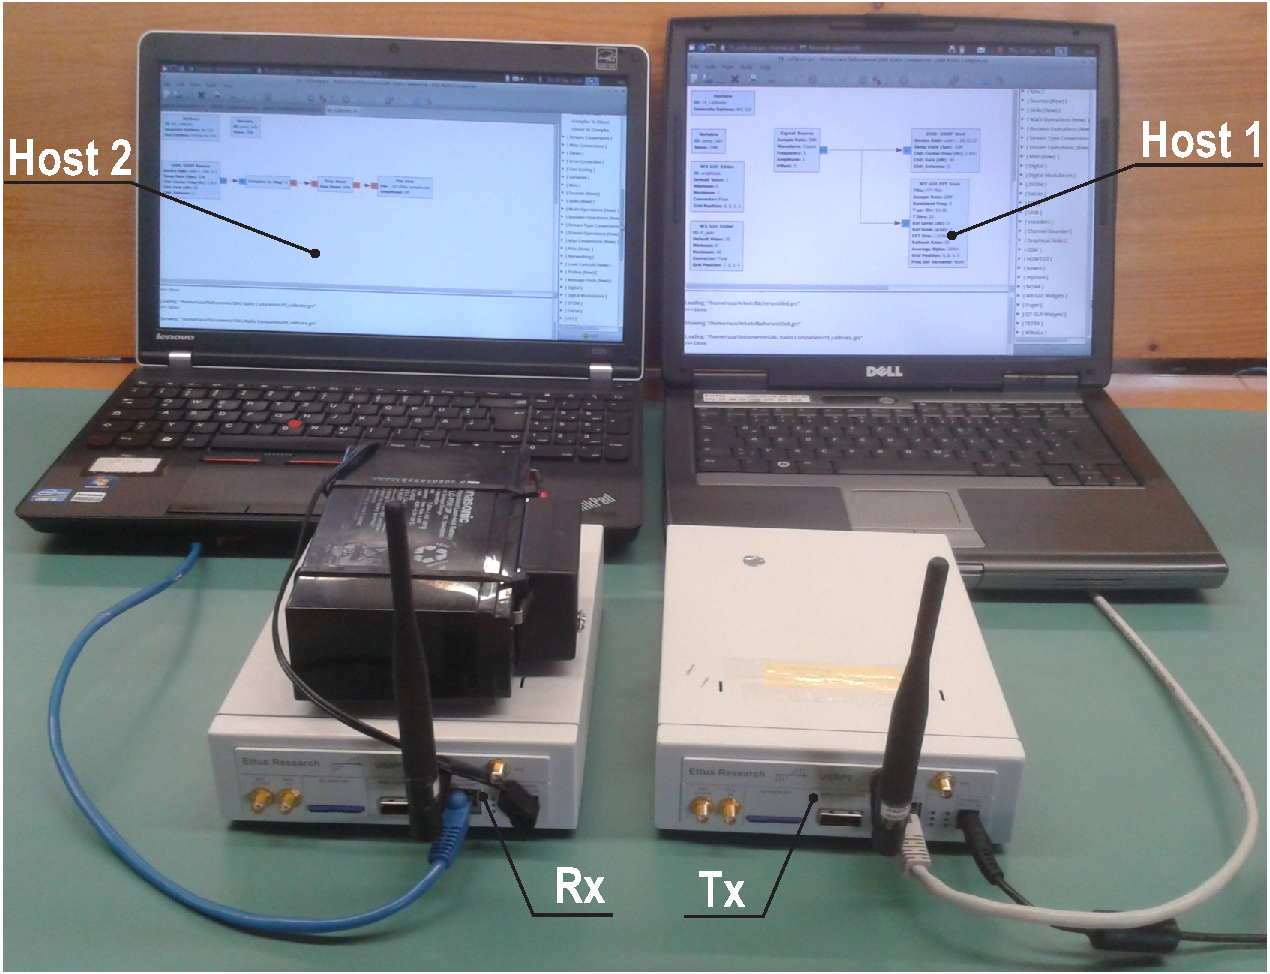
\includegraphics[width = 0.8\columnwidth]{../kapitel05/figures/setup}
%        \caption{Hardware setup.}
%        \label{fig:hw_setup}
%\end{figure}
%
%\subsection{Analysis}
%
%\subsubsection{\ac{IC} at PR}
%
%\begin{table}
%\renewcommand{\arraystretch}{1.3}
%\caption{Parameters and MSE of the $F_{I}$ modeled using Rayleigh and Nakagami-$m$ distribution for different PR positions}
%\label{tb:MSE_II}
%\centering
%\begin{tabular}{c||c|c}
%\hline
%\bfseries Outdoor & \bfseries Rayleigh (\ref{eq:expo}) & \bfseries Nakagami-$m$ (\ref{eq:gamma}) \\
%\bfseries Position & [MSE, $\widehat{\bar{\gamma}}]$ & [MSE, $(\widehat{m}, \widehat{\bar{\gamma}}$)] \\
%\hline\hline
%PR1 & $[3.84 \cdot 10^{-4}, 2.66 \cdot 10^{2} ]$  & $[1.74 \cdot 10^{-4} , (1.13, 2.66 \cdot 10^{2})] $ \\ \hline
%PR2 & $[2.75 \cdot 10^{-4}, 4.89 \cdot 10^{2}]$  & $[2.40 \cdot 10^{-4} , (0.98, 4.89 \cdot 10^{2})] $ \\ \hline
%PR3 & $[2.75 \cdot 10^{-4}, 57.34]$  & $[2.31 \cdot 10^{-4} , (1.11, 57.34)] $ \\ \hline
%PR4 & $[9.36 \cdot 10^{-4}, 94.20]$  & $[2.18 \cdot 10^{-4} , (1.25, 94.20)] $ \\ \hline
%\end{tabular}
%\end{table}
%
%
%\subsubsection{\ac{CC} at ID}
%
%\begin{figure}%
%\centering
%\begin{tikzpicture}[scale = 1.2]
%\node[anchor=south west,inner sep=0] (image) at (0,0)
%{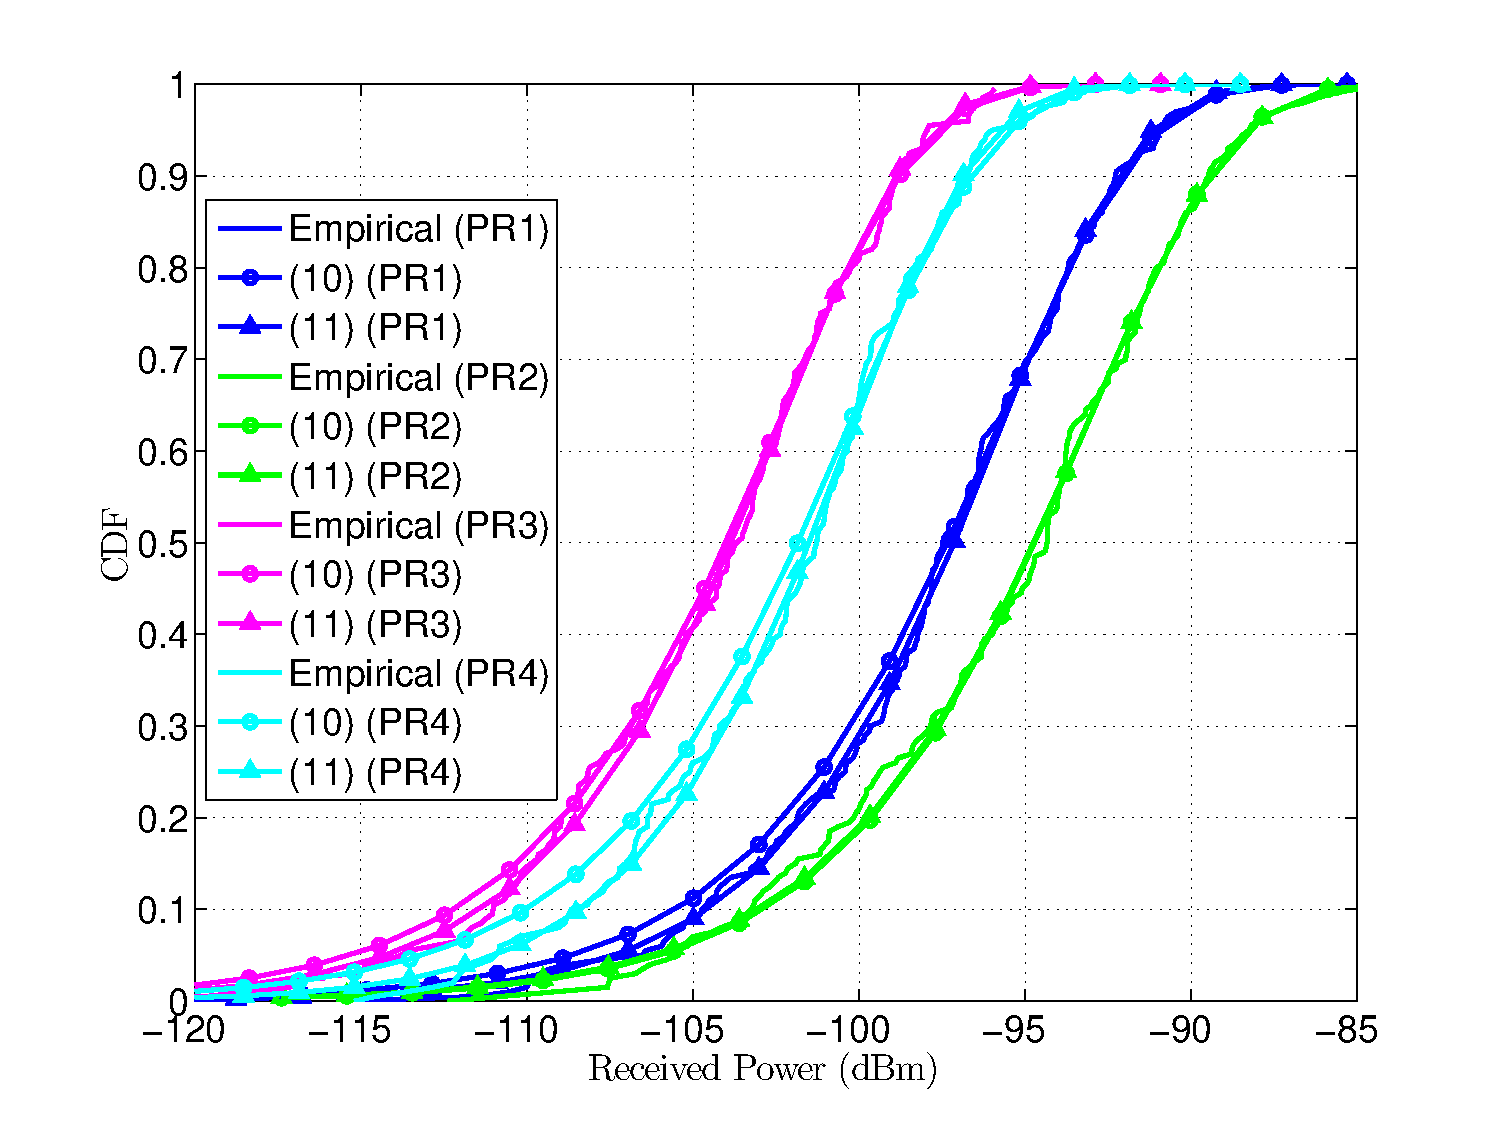
\includegraphics[trim=1.5cm 0.4cm 1.45cm 1.2cm,clip=true,width=\columnwidth]{../kapitel05/figures/Interference_CDF_ana_vs_sim_indoor_outdoor}};
%\begin{scope}[x={(image.south east)},y={(image.north west)}]
%\draw  (0.832,0.99) node[above=-0.1pt, font=\small] {$I_{\text{th}}$};
%\draw  (.97,0.898) node[right=-2.2pt, font=\small] {$\epsilon_{\text{I,out}}$};
%\draw[black,thick,<->] (0.97,0.898) --  node[right=-2.2pt, font=\small] {$\epsilon_{\text{I,out}}$} (0.97,0.985);
%\draw [thick] (0.831,0.985) -- (0.831,0.096);
%\draw [thick] (0.08,0.898) -- (0.956,0.898);
%
%%Select channels for based on Interference Constraint   
%\draw (0.675,0.85) ellipse(24pt and 5pt)  node[left=28pt, font=\small] {IC};
%\draw[help lines,xstep=.1,ystep=.1] (0,0) grid (1,1);
%\foreach \x in {0,1,...,9} { \node [anchor=north] at (\x/10,0) {0.\x}; }
%\foreach \y in {0,1,...,9} { \node [anchor=east] at (0,\y/10) {0.\y}; }
%\end{scope}
%\end{tikzpicture}
%\caption{Interference distribution function at different PR positions.}
%\label{subfig:indoor-outdoor}
%\end{figure}
%
%\begin{figure}
%\centering
%\begin{tikzpicture}[scale = 1.2]
%\node[anchor=south west,inner sep=0] (image) at (0,0)
%{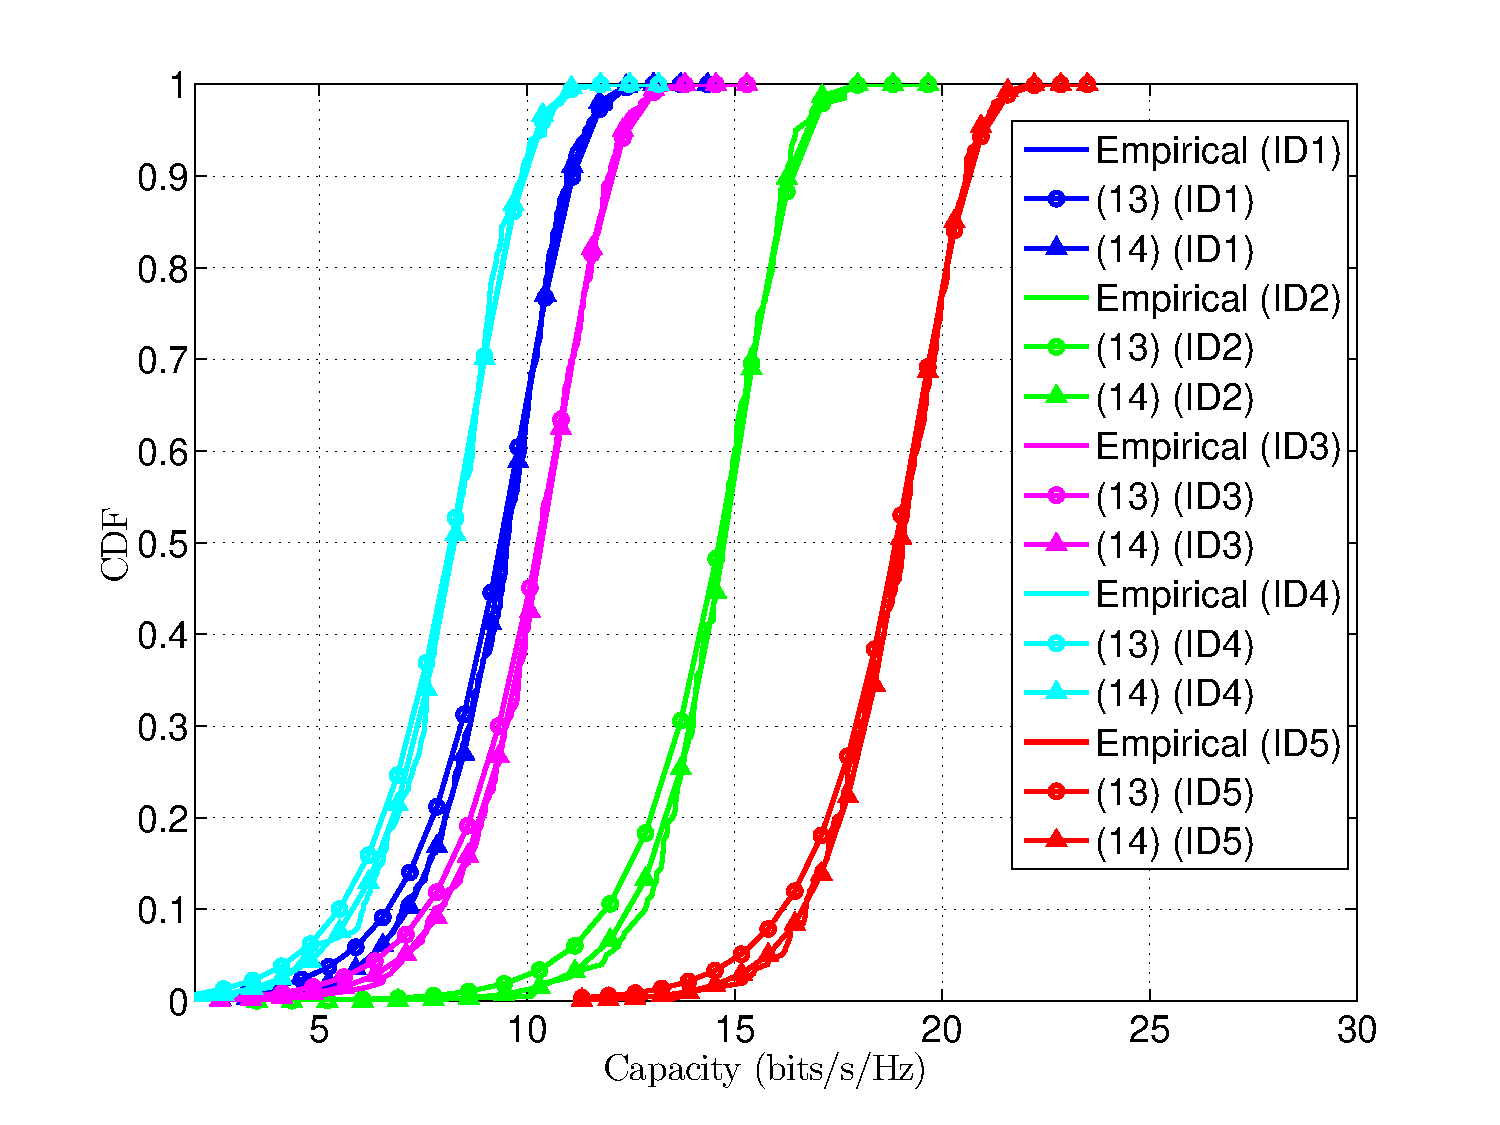
\includegraphics[trim=1.5cm 0.4cm 1.45cm 1.2cm,clip=true,width=\columnwidth]{../kapitel05/figures/Capacity_CDF_ana_vs_sim_indoor_indoor}};
%\begin{scope}[x={(image.south east)},y={(image.north west)}]
%\draw  (0.255,0.99) node[above=-0.1pt, font=\small] {$C_{\text{th}}$};
%\draw  (.97,0.178) node[right=-2.2pt, font=\small] {$\epsilon_{\text{C,out}}$};
%\draw[black,thick,<->] (0.97,0.095) --  node[right=-2.2pt, font=\small] {$\epsilon_{\text{C,out}}$} (0.97,0.186);
%\draw [thick] (0.255,0.985) -- (0.255,0.096);
%\draw [thick] (0.08,0.186) -- (0.956,0.186);
%Select channels for based on Capacity Constraint       
%\draw (0.48,0.58) ellipse (38pt and 5pt)  node[right=48 pt, font=\small] {CC};
%\draw[help lines,xstep=.1,ystep=.1] (0,0) grid (1,1);
%\foreach \x in {0,1,...,9} { \node [anchor=north] at (\x/10,0) {0.\x}; }
%\foreach \y in {0,1,...,9} { \node [anchor=east] at (0,\y/10) {0.\y}; }
%\end{scope}
%\end{tikzpicture}
%\label{subfig:indoor-indoor}
%\end{figure}
%
%\begin{table}
%\renewcommand{\arraystretch}{1.3}
%\caption{Parameters and MSE of the $F_{C}$ modeled using Rayleigh and Nakagami-$m$ distribution for different ID positions}
%\label{tb:MSE_IO}
%\centering
%\begin{tabular}{c||c|c}
%\hline
%\bfseries Indoor & \bfseries Rayleigh (\ref{eq:expo}) & \bfseries Nakagami-$m$ (\ref{eq:gamma}) \\
%\bfseries Position & [MSE, $\widehat{\bar{\gamma}}]$ & [MSE, $(\widehat{m}, \widehat{\bar{\gamma}}$)] \\
%\hline\hline
%ID1 & $[1.11 \cdot 10^{-3}, 9.52 \cdot 10^{2}]$  & $[1.74 \cdot 10^{-4} , (1.23, 9.52 \cdot 10^{2})] $ \\ \hline
%ID2 & $[1.60 \cdot 10^{-3}, 3.65 \cdot 10^{4}]$  & $[3.39 \cdot 10^{-4} , (1.28, 3.65 \cdot 10^{4})] $ \\ \hline
%ID3 & $[5.79 \cdot 10^{-4}, 1.79 \cdot 10^{2}]$  & $[1.35 \cdot 10^{-4} , (1.17, 1.79 \cdot 10^{2})] $ \\ \hline
%ID4 & $[9.35 \cdot 10^{-4}, 4.13 \cdot 10^{2}]$  & $[3.05 \cdot 10^{-4} , (1.16, 4.13 \cdot 10^{2})] $ \\ \hline
%ID5 & $[7.54 \cdot 10^{-4}, 6.99 \cdot 10^{4}]$  & $[2.96 \cdot 10^{-4} , (1.23, 6.99 \cdot 10^{4})] $ \\ \hline
%\end{tabular}
%\end{table}
%
%
%\begin{table}[!h]
%\renewcommand{\arraystretch}{1.3}
%\caption{Cognitive relay implementing AND rule for different PR and ID positions}
%\label{tb:BDecisions}
%\centering
%\begin{tabular}{c||c|c|c|c}
%\hline
%\bfseries & PR1 & PR2 & PR3 & PR4 \\
%\hline\hline
%ID1 & 1 $\cdot$ 0 = 0 & 0 $\cdot$ 0 = 0 & 1 $\cdot$ 0 = 0 & 1 $\cdot$ 0 = 0 \\ \hline
%ID2 & 1 $\cdot$ 1 = 1 & 0 $\cdot$ 1 = 0 & 1 $\cdot$ 1 = 1 & 1 $\cdot$ 1 = 1 \\ \hline
%ID3 & 1 $\cdot$ 1 = 1 & 0 $\cdot$ 1 = 0 & 1 $\cdot$ 1 = 1 & 1 $\cdot$ 1 = 1 \\ \hline
%ID4 & 1 $\cdot$ 0 = 0 & 0 $\cdot$ 0 = 0 & 1 $\cdot$ 0 = 0 & 1 $\cdot$ 0 = 0 \\ \hline
%ID5 & 1 $\cdot$ 1 = 1 & 0 $\cdot$ 1 = 0 & 1 $\cdot$ 1 = 1 & 1 $\cdot$ 1 = 1 \\ \hline
%\end{tabular}
%\end{table}




